
\chapter{Рекуррентные соотношения для коэффициентов ветвления представлений аффинных алгебр Ли}
\label{cha:affine-lie-algebras}

В главе \ref{cha:CFT} мы показали, что для построения модулярно-инвариантных статсумм и в процессе изучения coset-моделей возникает проблема ветвления для аффинных алгебр Ли.  В данной главе мы выводим рекуррентные соотношения на коэффициенты ветвления, которые являеются важнейшим инструментом данной диссертации. Эти соотношения получены нами в работе \cite{2010arXiv1007.0318L}.

Существуют различные подходы к вычислению коэффициентов ветвления. Некоторые из них используют резольвенту Бернштейна-Гельфанда-Гельфанда \cite{bernstein1975differential} (См. главу \ref{cha:BGG}, алгоритм вычислений описан в работах \cite{kac1990idl},\cite{wakimoto2001idl}), ряды функций Шура \cite{fauser2006new}, когомологии БРСТ  \cite{Hwang:1994yr}, формулы Каца-Петерсона  \cite{kac1990idl,quella2002branching} или комбинаторные методы \cite{feigin707principal}.

В этой главе мы доказываем, что для произвольной редуктивной подалгебры коэффициенты ветвления описываются набором рекуррентных соотношений и существует эффективный и простой алгоритм для пошагового решения этих соотношений. Общая идея похожа на подход, предложенный в работе  \cite{ilyin812pbc} для максимальных вложений. Но в данном случае алгоритм существенно отличается, так как использует новые свойства сингулярных весов для работы с произвольными редуктивными вложениями $\af \rightarrow \gf$.

При этом важно рассматривать подалгебру  $\af$ вместе с ее ``ортогональным партнером'' $\afb\subset \gf$. 
Для любой редуктивной подалгебры $\af$ подалгебра $\afb$ регулярна и редуктивна. 

Для модуля старшего веса  $L^{\left( \mu \right)}$ и ортогональной пары подалгебр $\left(  \af, \afb \right)$ мы рассматриваем так называемый сингулярный элемент  $\Psi^{\left( \mu \right)}$ (числитель в формуле Вейля для характеров
$ch\left( L^{\mu }\right) =\frac{\Psi ^{\left( \mu \right) }}{\Psi ^{\left( 0\right) }}$,
см., например, \cite{humphreys1997introduction}), 
знаменатель Вейля $\Psi ^{\left( 0\right) }_{\afb}$ и проекцию
$\Psi ^{\left( \mu \right) }_{\left(  \af, \afb \right)}
=\pi_{\af}\frac{\Psi ^{\left( \mu \right) }_{\gf}}{\Psi ^{\left( 0\right) }_{\afb}}$.

Мы доказываем, что для произвольного $\hf$-диагонализующего модуля старшего веса $L^{\left( \mu \right)}$ и ортогональной пары $\left(  \af, \afb \right)$ элемент
$\Psi ^{\left( \mu \right) }_{\left(  \af, \afb \right)}$ допускает разложение на множество числителей Вейля $\Psi ^{\left( \mu \right) }_{ \afb }$ модулей подалгебры $\afb$.
Это разложение дает возможность построить рекуррентное соотношение для коэффициентов ветвления, соответствующих вложению $\af \rightarrow \gf $. Рекуррентное соотношение формулируется с использованием особого элемента  $\Gamma_{\af \rightarrow \gf}$ групповой алгебры
$\mathcal{E}\left( \gf \right)$, который мы называем ``веером вложения''. 
Применение этих инструментов позволяет нам сформулировать простой и явный алгоритм для вычисления коэффициентов ветвления, который может быть использован в случае произвольных (максимальных и не максимальных) подалгебр конечномерных и аффинных алгебр Ли. 
В случае максимального вложения веер имеет простую форму, сингулярный элемент становится тривиальном $\Psi ^{\left( \mu \right) }_{\left(  \af, \afb \right)}=\Psi ^{\left( \mu \right) }_{\left(  \gf\right)}$ и мы восстанавливаем соотношения, полученные ранее в работе \cite{ilyin812pbc}.

Также мы показываем, что предложенный алгоритм эффективен и может использоваться при изучении конформных вложений и coset-моделей в рациональной конформной теории поля.

В следующем разделе \ref{sec:intro-simple-lie-algebras} мы определяем аффинные алгебры Ли и приводим основные определения в теории представлений.  Заодно мы фиксируем обозначения. Затем в разделе \ref{sec:branching} мы выводим формулы разложения, основывающиеся на аномальных коэффициентах ветвления и описываем алгоритм редукции интегрируемых модулей старшего веса $L_{\mathfrak{g}}$ по отношению к редуктивной подалгебре  $\mathfrak{a}\subset \mathfrak{g}$ (см. секцию \ref{sec:algorithm}). В разделе \ref{sec:branching-examples} мы представляем различные примеры применения алгоритма для конечномерных (\ref{sec:finite-dimens-lie}) и аффинных алгебр Ли и обсуждаем их роль в моделях конформной теории поля (\ref{sec:phys-appl}). Выводы к главе изложены в разделе \ref{sec:conclusion}. В следующей главе \ref{cha:BGG} мы показываем связь процедуры редукции с обобщенной резольвентой Бернштейна-Гельфанда-Гельфанда.  Реализация алгоритма на языке {\it Mathematica} и дополнительные примеры машинных вычислений описаны в главе  \ref{cha:computational-methods}. 

%%  \subsubsection{Notation}
%%  \label{sec:notation}
%%  
%%  Consider affine Lie algebras $\gf$ and $\af$ with
%%  underlying finite-dimensional subalgebras $\go$ and $%
%%  \ao$ and an injection $\af\longrightarrow \frak{g%
%%  }$ such that $\af$ is a reductive subalgebra $\frak{a\subset g}$ with
%%  correlated root spaces: $\hf_{\af}^{\ast }\subset \hf_{\frak{g%
%%  }}^{\ast }$ and $\hf_{\ao}^{\ast }\subset \frak{h%
%%  }_{\go}^{\ast }$\
%%  .
%%  We use the following notations:
%%  
%%  $L^{\mu }$\ $\left( L_{\af}^{\nu }\right) $\ --- the integrable module
%%  of $\gf$ with the highest weight $\mu $\ ; (resp. integrable $\af$
%%  -module with the highest weight $\nu $ );
%%  
%%  $r$ , $\left( r_{\af}\right) $ --- the rank of the algebra $\gf$ $%
%%  \left( \mbox{resp. }\af\right) $ ;
%%  
%%  $\Delta $ $\left( \Delta _{\af}\right) $--- the root system; $\Delta
%%  ^{+} $ $\left( \mbox{resp. }\Delta _{\af}^{+}\right) $--- the positive
%%  root system (of $\gf$ and $\af$ respectively);
%%  
%%  $\mathrm{mult}\left( \alpha \right) $ $\left( \mathrm{mult}_{\af}\left(
%%  \alpha \right) \right) $ --- the multiplicity of the root $\alpha$ in $\Delta
%%  $ (resp. in $\left( \Delta _{\af}\right) $);
%%  
%%  $\co{\Delta}$ , $\left( \co{\Delta _{\af}}%
%%  \right)$ --- the finite root system of the subalgebra $\co{%
%%  \gf}$ (resp. $\co{\af}$);
%%  
%%  $\mathcal{N}^{\mu }$ , $\left( \mathcal{N}_{\af}^{\nu }\right) $ --- the
%%  weight diagram of $L^{\mu }$ $\left( \mbox{resp. }L_{\af}^{\nu }\right)
%%  $ ;
%%  
%%  $W$ , $\left( W_{\af}\right) $--- the corresponding Weyl group;
%%  
%%  $C$ , $\left( C_{\af}\right) $--- the fundamental Weyl chamber;
%%  
%%  $\bar{C}, \left(\bar{C_{\mathfrak{a}}}\right)$ --- the closure of the fundamental Weyl chamber;
%%  
%%  $\rho $\ , $\left( \rho _{\af}\right) $\ --- the Weyl vector;
%%  
%%  $\epsilon \left( w\right) :=\det \left( w\right) $ ;
%%  
%%  $\alpha _{i}$ , $\left( \beta _{j}\right) $ --- the $i
%%  $-th (resp. $j$-th) basic root for $\gf$ $\left( \mbox{resp. }\af%
%%  \right) $; $i=0,\ldots ,r$,\ \ $\left( j=0,\ldots ,r_{\af}\right) $;
%%  
%%  $\delta $ --- the imaginary root of $\gf$ (and of $\af$ if any);
%%  
%%  $\alpha _{i}^{\vee }$ , $\left( \beta _{j}^{\vee
%%  }\right) $--- the basic coroot for $\gf$ $\left( \mbox{resp. }\af%
%%  \right) $ , $i=0,\ldots ,r$ ;\ \ $\left( j=0,\ldots ,r_{\af}\right) $;
%%  
%%  $\co{\xi }$ , $\co{\xi _{\left( \af\right) }}$
%%  --- the finite (classical) part of the weight $\xi \in P$ , $\left( \mbox{%
%%  resp. }\xi _{\left( \af\right) }\in P_{\af}\right) $;
%%  
%%  $\lambda =\left( \co{\lambda };k;n\right) $ ---
%%  decomposition of the affine weight $\lambda$ indicating the finite
%%  part $\co{\lambda }$, the level $k$ and the grade $n$;
%%  
%%  $P$ $\left( \mbox{resp. } P_{\af}\right) $ \ --- the weight lattice;
%%  
%%  $m_{\xi }^{\left( \mu \right) }$ , $\left( m_{\xi }^{\left( \nu \right)
%%  }\right) $ --- the multiplicity of the weight $\xi \in P$ \ $\left( \mbox{%
%%  resp. }\in P_{\af}\right) $ in the module $L^{\mu }$ , (resp. $\xi \in
%%  L_{\af}^{\nu } $);
%%  
%%  $ch\left( L^{\mu }\right) $ $\left( \mbox{resp. }ch\left( L_{\af}^{\nu
%%  }\right) \right) $--- the formal character of $L^{\mu }$ $\left( \mbox{resp. }%
%%  L_{\af}^{\nu }\right) $;
%%  
%%  $ch\left( L^{\mu }\right) =\frac{\sum_{w\in W}\epsilon (w)e^{w\circ (\mu
%%  +\rho )-\rho }}{\prod_{\alpha \in \Delta ^{+}}\left( 1-e^{-\alpha }\right) ^{%
%%  \mathrm{{mult}\left( \alpha \right) }}}$ --- the Weyl-Kac formula;
%%  
%%  $R:=\prod_{\alpha \in \Delta ^{+}}\left( 1-e^{-\alpha }\right) ^{\mathrm{{%
%%  mult}\left( \alpha \right) }}\quad $
%%  $\left( \mbox{resp. }R_{\af}:=\prod_{\alpha \in \Delta _{%
%%  \af}^{+}}\left( 1-e^{-\alpha }\right) ^{\mathrm{mult}_{\af}\mathrm{%
%%  \left( \alpha \right) }}\right) $--- the Weyl denominator.
%%  
%%  
%%  
\section{Простые алгебры Ли, алгебра петель, центральные расширения и аффинные алгебры Ли}

\label{sec:intro-simple-lie-algebras}
\begin{definition}
{\it Алгебра Ли $\gf$} -- это векторное пространство с билинейной операцией $[\cdot,\cdot]:\gf\otimes\gf\to \gf$, которая называется  {\it скобкой Ли или коммутатором}. Если выбрать некоторый базис  $X_{i}$ в $\gf$, то коммутационные соотношения можно задать при помощи  {\it структурных констант} $C_{ijk}$:
\begin{equation}
  \label{eq:1}
  [X^{i},X^{j}]=\sum_{k} C^{ij}_{k} X^{k}
\end{equation}
  
\end{definition}

Алгебра Ли называется {\it простой} если она не содержит нетривиальных идеалов относительно коммутатора. {\it Полупростая} алгебра Ли -- это прямая сумма простых алгебр Ли. 

{\it Подалгеброй Картана}  $\hfg$ называется нильпотентная подалгебра алгебры $\gf$, совпадающая со своим нормализатором. Мы обозначаем элементы базиса в $\hfg$ через $H^{i}$.

Форма Киллинга на  $\gf$ порождает невырожденную билинейную форму $(\cdot,\cdot)$ на подалгебре Картана $\hfg$, позволяющую идентифицировать $\hfg$ с подпространством дуального пространства  $\hfg^{*}$ линейных функционалов на $\hfg$. {\it Веса}  -- это элементы  $\hfg^{*}$, мы обозначаем их греческими буквами $\mu,\nu, \omega, \lambda\dots$


Коммутационные соотношения  (\ref{eq:1}) можно записать в компактной форме, если выбрать базис специальным образом. Такой базис описывается корневой системой, которая определяется в разделе \ref{sec:weights-roots} (Смотри также \cite{humphreys1997introduction,humphreys1992reflection}).

Чтобы определить аффинные алгебры нам нужно обсудить процедуру центрального расширения алгебры Ли.
Напомним несколько определений (см \cite{fuks1986cohomology},\cite{fuks1984}, \cite{feigin1988}).
\begin{definition}
\label{def:1}
Будем рассматривать алгебру Ли $\gf$ над полем $k=\mathbb{C},\mathbb{R}$. Векторное пространство $A$ над полем $k$ называется {\it модулем над $\gf$} или {\it $\gf$-модулем}, если задано билинейное отображение $\mu:\gf\times A\to A$, такое что $\mu([X,Y],a)=\mu(X,\mu(Y,a))-\mu(Y,\mu(X,a))$ для $X,Y\in \gf, a\in A$. Далее мы будем опускать символ $\mu$ и писать $X a= \mu(X,a)$.
\end{definition}
\begin{definition}
  {\it $n$-мерная коцепь с коэффициентами в $A$} -- это кососимметричный $n$-линейный функционал на $\gf$ со значениями в $A$. Пространство $n$-коцепей $C^{n}(\gf;A)=\mathrm{Hom}(\wedge^{n}\gf;A)$.
\end{definition}
Заметим, что элементы $\gf$ действуют на $C^{n}(\gf;A)$.
\begin{definition}
  Внешний дифференциал $d=d_{n}:C^{n}(\gf;A)\to C^{n+1}(\gf;A)$ определяется формулой
  \begin{multline}
    \label{eq:68}
    (dc) (X_{1},\dots, X_{n+1})=\sum_{1\leq s<t\leq n+1} (-1)^{s+t-1} c([X_{s},X_{t}],X_{1},\dots,\hat X_{s},\dots,\hat X_{t},\dots X_{n+1})\\
    +\sum_{1\leq s\leq n+1} (-1)^{s}X_{s} c(X_{1},\dots \hat X_{s},\dots X_{n+1})
  \end{multline}
\end{definition}
Нетрудно проверить, что последовательность
\begin{equation}
  \label{eq:40}
  \dots\stackrel{d_{n}}{\longleftarrow} C^{n}(g;A)\stackrel{d_{n-1}}{\longleftarrow} C^{n-1}(\gf;A)\leftarrow \dots \leftarrow C^{1}(\gf;A) \stackrel{d_{0}}{\longleftarrow} C^{0}(\gf;A)\leftarrow 0
\end{equation}
точна.Тогда $\{C^{n}(\gf;A),d_{n}\}=C^{*}(\gf;A)$ есть комплекс.
\begin{definition}
Соответствующие когомологии называются {\it когомологиями алгебры $\gf$ с коэффициентами в $A$} и обозначаются через $H^{n}(\gf;A)=\mathrm{Ker}\; d_{n}/\mathrm{Im}\; d_{n-1}$. 
  
\end{definition}
Заметим, что поле $k$ может рассматриваться как тривиальный $\gf$-модуль. В этом случае второй член в формуле \eqref{eq:1} исчезает и используют сокращенные обозначения $C^{n}(\gf), H^{n}(\gf)$.
\begin{definition}
  Определим, заодно, и гомологии. Пространство $n$-мерных цепей $C_{n}(\gf;A)=A\otimes \wedge^{n}\gf$, дифференциал $\partial=\partial_{n}:C_{n}(\gf;A)\to C_{n-1}(\gf;A)$ определяется формулой
  \begin{multline}
    \label{eq:98}
    \partial(a\otimes (X_{1}\wedge \dots \wedge X_{n})) =\\ \sum_{1\leq s<t\leq n+1} (-1)^{s+t-1} a\otimes ([X_{s},X_{t}]\wedge X_{1} \wedge\dots\wedge\hat X_{s}\wedge \dots\wedge \hat X_{t}\wedge \dots\wedge X_{n+1})\\
    +\sum_{1\leq s\leq n+1} (-1)^{s}(X_{s} a)\otimes (X_{1}\wedge\dots\wedge \hat X_{s}\wedge\dots\wedge X_{n+1})
  \end{multline}
  Аналогично определяется точная последовательность, комплекс и группа гомологий $H_{n}(\gf;A)$.
\end{definition}
\begin{definition}
  {\it Одномерным центральным расширением алгебры $\gf$ } называется точная последовательность
  \begin{equation}
    \label{eq:62}
    0\to k \to \tilde \gf\to \gf\to 0,
  \end{equation}
  такая что образ $k\to \tilde\gf$ содержится в центре $\tilde\gf$.
\end{definition}
Заметим, что всякий 2-коцикл $c\in C^{2}(\gf;A), \; dc=0$ определяет центральное расширение $\gf$:
\begin{equation}
  \label{eq:64}
  0\to k\stackrel{\lambda\to (0,\lambda)}{\longrightarrow}\tilde\gf=\gf\oplus k \stackrel{(X,\lambda)\to X}{\longrightarrow} \gf\to 0
\end{equation}
Скобка Ли в алгебре $\tilde\gf$, которая равна $\gf\oplus k$ как векторное пространство, определяется равенством
\begin{equation}
  \label{eq:103}
  [(X,\lambda),(Y,\mu)]=([X,Y],c(X,Y))
\end{equation}
Тождество Якоби для такой скобки равносильно тому, что $c$\; --- 2-коцикл. Когомологичным коциклам отвечают эквивалентные расширения. 

Два расширения $\tilde \gf$ и $\tilde{\tilde\gf}$ называются эквивалентными, если существует изоморфизм $I:\tilde\gf\to \tilde{\tilde \gf}$ такой, что диаграмма коммутирует:
\begin{equation}
  \label{eq:104}
  \begin{diagram}
    \node 0 \arrow{e,t}{}  \node{\gf} \arrow{e,t}{} \arrow{s,l}{id} \node{\tilde\gf}\arrow{s,l}{I} \arrow{e,t}{} \node{k}\arrow{s,r}{id} \arrow{e,t}{} \node{0}\\
    \node 0 \arrow{e,t}{}  \node{\gf} \arrow{e,t}{} \node{\tilde{\tilde\gf}} \arrow{e,t}{} \node{k} \arrow{e,t}{} \node{0}
  \end{diagram}
\end{equation}
%% \begin{exercise}
%%  Построить изоморфизм $I$.   
%% \end{exercise}


Таким образом пространство $H^{2}(\gf)$ -- это множество классов 1-мерных центральных расширений $\gf$. Нуль в $H^{2}(\gf)$  соответствует тривиальному расширению. 

Для алгебры Витта \eqref{eq:2} существует коцикл
\begin{equation}
  \label{eq:105}
  c(l_{n},l_{m})=\frac{1}{12}(m^{3}-m)\delta_{-n,m}
\end{equation}
%% \begin{exercise}
%%   Проверить, что $c$ -- коцикл алгебры Витта. 
%% \end{exercise}
Соответствующее центральное расширение алгебры Витта называется алгеброй Вирасоро. Коммутационные соотношения этой алгебры имеют вид
\begin{eqnarray}
  \label{eq:106}
  [L_{n},c]=0\\
  \left[L_{n},L_{m}\right]=(n-m)L_{n+m} +\frac{c}{12} (m^{3}-m) \delta_{-n,m}
\end{eqnarray}
Можно показать, что $H^{2}(Witt)\cong \mathbb{C}$ и все нетривиальные коциклы пропорциональны $c$. 
(Доказательство есть в \cite{fuks1986cohomology}, \cite{schottenloher2008mathematical}).

{\it Алгебра петель} $L\gf=\gf\otimes \mathbb{C}[t,t^{-1}]$, соответствующая полупростой алгебре Ли $\gf$, определяется коммутационными соотношениями
\begin{equation}
  \label{eq:108}
  [X^{i}t^{n},X^{j}t^{m}]=t^{n_+m}\sum_{k}C^{ij}_{k}X^{k}
\end{equation}
Центральное расширение алгебры петель ведет к возникновению дополнительного члена
\begin{equation}
  \label{eq:112}
   [X^{i}t^{n}+\alpha c,X^{j}t^{m}+\beta c]=t^{n+m}\sum_{k}C^{ij}_{k}X^{k}+(X^{i},X^{j})n\delta_{n+m,0}c
\end{equation}
Эта алгебра $\hat\gf=\gf\otimes\mathbb{C}[t,t^{-1}]\oplus\mathbb{C}c$ называется (не скрученной)  {\it аффинной алгеброй Ли} \cite{kac1990idl}, \cite{wakimoto2001idl,wakimoto2001lectures}, \cite{kass1990ala}.

\subsection{Модули, веса и корни}
\label{sec:weights-roots}

Пусть $\gf$ -- конечномерная или аффинная алгебра Ли. Мы ввели модули алгебры $\gf$ в определении \ref{def:1}. Широко используется альтернативный термин {\it представление}.

%%    $\gf$-модулем называется векторное пространство $V$ с билинейным отображением $\gf \times V\to V$, таким, что выполнено равенство
%%  \begin{equation}
%%    \label{eq:130}
%%    [x,y]\cdot v = x\cdot(y\cdot v) - y\cdot(x\cdot v), \quad \mbox{for}\; x,y\in \gf, v\in V
%%  \end{equation}
\begin{definition}
Представление алгебры  $\gf$ на векторном пространстве $V$ называется гомоморфизм $\gf\to gl(V)$ из $\gf$ в алгебру Ли эндоморфизмов векторного пространства $V$, где скобка задана коммутатором:
\begin{equation}
  \label{eq:113}
  [x,y]\cdot v = x\cdot(y\cdot v) - y\cdot(x\cdot v), \quad \mbox{для}\; x,y\in \gf, v\in V  
\end{equation}

\end{definition}

В произвольном представлении операторы, соответствующие генераторам подалгебры Картана $H^{i}$ можно одновременно диагонализовать путем специального выбора базиса
 $\{v_{j}\}$ в $V$:
\begin{equation}
  \label{eq:114}
  H^{i}\cdot v_{j}=\nu_{j}^{i}v_{j}
\end{equation}
Собственные значения $\nu^{i}_{j}$ генераторов Картана на элементе базиса $v_{j}$ определяют вес  $\nu_{j}\in \hfg^{*}$, такой, что $\nu_{j}(H^{i})=\nu_{j}^{i}$. Вектор $v\in V$ называется весовым вектором веса  $\lambda$, если $H v=\lambda_{j}(H)v,\; \forall H\in \hf$. Весовое подпространство состоит из всех весовых векторов $V_{\lambda}=\{v\in V: H v=\lambda_{j}(H)v,\; \forall H\in \hf\}$. Кратностью веса  $m_{\lambda}=\mathrm{mult}(\lambda)=\mathrm{dim} V_{\lambda}$ называется размерность весового подпространства.

Структура модуля определяется набором весов, так как действие генераторов $E^{\alpha}$ на весовых векторах дается выражением
\begin{equation}
  \label{eq:115}
  E^{\alpha}\cdot v_{\lambda} \propto v_{\lambda+\alpha}
\end{equation}
Структуру модуля можно записать в виде формального характера
\begin{equation}
  \label{eq:116}
  \mathrm{ch}V=\sum_{\lambda}m_{\lambda} e^{\lambda}
\end{equation}
Характер  $\mathrm{ch}V\in \mathcal{E}$ -- это элемент алгебры  $\mathcal{E}$, порожденной формальными экспонентами весов. Характер можно специализировать --- взять его значение на некотором элементе $\xi\in\hf$.

Алгебра Ли является собственным модулем по отношению к специальному представлению, называющемуся присоединенном. Действие генераторов в этом представлении дается скобкой $ad_{X} Y=[X,Y]$. 
{\it Корни} -- это веса присоединенного представления алгебры $\gf$.  Они определяют коммутационные соотношения в алгебре следующим образом. Обозначим через $\Delta$ множество корней. Для каждого $\alpha\in \Delta$ существует корень  $-\alpha\in \Delta$ и генераторы $E^{\alpha}, E^{-\alpha}$, такие, что
\begin{align}
  \label{eq:63}
  &  [H^{i},E^{\alpha}]=\alpha^{i}E^{\alpha} \\
  &\left[E^{\alpha},E^{\beta}\right]=
  \begin{cases}
    N_{\alpha,\beta} E^{\alpha+\beta}, & \mbox{if}\; \alpha+\beta\in \Delta\\
    \frac{2}{(\alpha,\alpha)} \sum_{i}\alpha^{i} H^{i},&  \mbox{if}\; \alpha=-\beta\\
    0,&\mbox{в остальных случаях}
  \end{cases}
\end{align}

В корневой системе $\Delta$ можно выбрать множество положительных корней. Это подмножество  $\Delta^{+}\subset \Delta$, такое, что для любого корня $\alpha\in\Delta$ ровно один из корней $\alpha, -\alpha$ содержится $\Delta^{+}$ и для любых двух различных положительных корней $\alpha, \beta\in \Delta^{+}$, таких, что $\alpha+\beta\in \Delta$ их сумма тоже положительна $\alpha+\beta\in\Delta^{+}$.
Элементы множества $-\Delta^{+}$ называются отрицательными корнями.

Положительный корень называется {\it простым} если его нельзя представить в виде суммы положительных корней. Множество простых корней  $\Phi=\left\{\alpha_{i}\right\}$ является базисом в $\hfg^{*}$ и каждый корень может быть записан как сумма $\alpha=\sum_{i}n_{i}\alpha_{i}$, где все $n_{i}$ не отрицательны или не положительны одновременно. В случае конечномерной алгебры Ли  $\gf$ простые корни можно пронумеровать числами от  1 до ранга алгебры $i=1,\dots,r,\quad r=\mathrm{rank}(\gf)$. Такая нумерация порождает лексикографическое упорядочение корневой системы. Старший по отношению к этому упорядочению корень обозначается через $\theta=\sum_{i=1,\dots,r} a_i \alpha_i$, его координаты в базисе простых корней $a_i$ называются  {\it марками}. $\theta$ -- это старший вес присоединенного модуля (См. раздел \ref{sec:high-weight-modul}). {\it Ко-марками} называются числа, равные $a_i^{\vee}=\frac{(\alpha_i,\alpha_i)}{2} a_i$.

В аффинной алгебре Ли  $\hat\gf$ множество корней  $\Delta$ бесконечно, но набор простых корней  $\Phi$ конечен. Обозначим его элементы через $\alpha_{0},\dots \alpha_{r}$, где $r=\mathrm{rank}(\gf)$. Корни $\alpha_1,\dots, \alpha_r$ -- это корни соответствующей конечномерной алгебры Ли $\go$. Простой корень  $\alpha_0=\delta-\theta$ -- это разность  {\it мнимого корня} $\delta$ и $\theta$ -- старшего корня алгебры $\go$.
Заметим, что кратность корня  $\mathrm{mult}(\alpha)$ в случае аффинной алгебры Ли может быть больше единицы.

Подалгебра  $\bff_{+}\subset \gf$, порожденная генераторами $H^{i}, E^{\alpha}$, соответствующими положительным корням $\alpha\in \Delta^{+}$, называется подалгеброй Бореля.

{\it Параболическая подалгебра}  $\pf_{I}\supset \bff_{+}$ содержит подалгебру Бореля и порождена некоторым подмножеством простых корней  $\{\alpha_{j}:j\in I, I\subset \{1\dots r\}\}$. Она образована подмножеством генераторов  $\{H^{i}\}\cup \{E^{\alpha}:\alpha\in \Delta^{+}\}\cup \{E^{-\alpha}: \alpha\in\Delta^{+}, \alpha=\sum_{j\in I} n_{j} \alpha_{j}\}$.
{\it Регулярная подалгебра} $\af\subset\gf$ определяется корневой системой  $\Delta_{\af}$, множество простых корней которой  $\{\beta_{i}, i=1,\dots,r_{\af}\}$ является подмножеством множества $\{\alpha_{1},\dots,\alpha_{r}\}\cup \{-\theta\}$ корней алгебры $\gf$.

 {\it Группа Вейля} $W_{\gf}$ порождается отражениями $\{s_{i}:\hfg^{*}\to\hfg^{*}\}$, соответствующим простым корням $\{\alpha_{i}\}$:
\begin{equation}
  \label{eq:117}
  s_{i}\cdot\lambda=\lambda-\frac{2(\alpha_{i},\lambda)}{(\alpha_{i},\alpha_{i})}\alpha_{i}
\end{equation}
Корневая система и характеры представлений инвариантны относительно действия группы Вейля. Корневая система может быть восстановлена из множества простых корней в результате применения вейлевских отражений.

Группа Вейля конечна для конечномерных алгебр Ли и конечно порождена для аффинных алгебр Ли.

Рассмотрим действие элемента группы Вейля $s_{\alpha}s_{\alpha+\delta}$ аффинной алгебры Ли   $\hat\gf$, соответствующего простому корню  $\alpha$ конечномерной подалгебры Ли $\gf$. Из определения  \eqref{eq:117} легко видеть, что $s_{\alpha}s_{\alpha+\delta} \cdot \lambda=\lambda+\frac{2}{(\alpha,\alpha)}\alpha+\left(\frac{(\alpha,\alpha)}{2 (\lambda,\delta)}+(\lambda,\alpha)\right) \delta$. То есть группа Вейля для аффинной алгебры Ли может быть представлена как полупрямое произведение группы Вейля $W_{\gf}$ конечномерной подалгебры  $\gf$ и трансляций, соответствующих корням $\gf$. 

Элемент группы Вейля можно представить как произведение простых отражений различными способами. Число простых отражений в кратчайшей последовательности, представляющей элемент\; $w\in W_{\gf}$ называется {\it длиной}  $w$ и обозначается $l(w)$. Мы также используем обозначение $\epsilon(w)=(-1)^{l(w)}$ для четности числа отражений Вейля, порождающих $w$. 

Фундаментальная область $\bar{C}$ для действия группы Вейля $W_{\gf}$ на $\hfg^{*}$ описывается условием $\xi\in \bar{C}\Leftrightarrow (\xi,\alpha_{i})\geq 0$ для всех простых корней $\alpha_{i}$. Ее называют {\it главной камерой Вейля}. 

{\it Матрица Картана} $A$ строится из произведений простых корней
\begin{equation}
  \label{eq:118}
  A_{ij}=\frac{2(\alpha_{i},\alpha_{j})}{(\alpha_{j},\alpha_{j})}.
\end{equation}
Она может использоваться для компактного описания алгебры Ли и ее коммутационных соотношений в базисе Шевалле \cite{humphreys1997introduction}, \cite{fulton1991representation}, \cite{bourbaki2002lie}.

Форма, заданная матрицей Картана \eqref{eq:118} определяет базис, дуальный к базису простых корней.  Он называется  {\it базисом фундаментальных весов}. Мы обозначаем его элементы через $\omega_i$:
\begin{equation}
  \label{eq:20}
  \langle\omega_i,\alpha_j\rangle=\frac{2(\omega_{i},\alpha_{j})}{(\alpha_{j},\alpha_{j})}=\delta_{ij}
\end{equation}
Для конечномерной алгебры Ли существует $r$ фундаментальных весов $\omega_{i}$, $i=1,\dots, r$. Для аффинной алгебры Ли есть дополнительный фундаментальный вес $\omega_0=\lambda$, $(\lambda,\delta)=1, \; (\lambda,\lambda)=(\delta,\delta)=0$. Другие фундаментальные веса равны $\omega_i=a_i^{\vee} \omega_0 +\co{\omega_i}$, где $\co{\omega_i}$ -- это фундаментальные веса конечномерной подалгебры Ли $\gf$.

Сумма фундаментальных весов $\rho=\sum_{i} \omega_{i}$ называется {\it вектором Вейля} и играет большую роль в теории представлений.

\subsection{Модули старшего веса}
\label{sec:high-weight-modul}

Мы рассматриваем конечно-порожденные  $\gf$-модули $V$, такие, что $V=\bigoplus_{\xi\in \hfg^{*}} V_{\xi}$, где каждое подпространство $V_{\xi}$ конечномерно и существует конечный набор весов $\lambda_{1},\dots \lambda_{s}$, порождающий весовую систему модуля $V$. То есть, если $\mathrm{dim}V_{\xi}\neq 0$, то $\xi=\lambda_{i}-\sum_{k=1,\dots, r} n_{k}\alpha_{k}$, где $n_{k}\in \mathbb{Z}_{+}$ (См.  \cite{humphreys2008representations}, \cite{carter2005lie}).

Модули старшего веса содержат единственный старший вес $\mu$ и все остальные веса в них могут быть получены вычитанием линейных комбинаций простых корней $\lambda=\mu-n_{1}\alpha_{1}-\dots-n_{r}\alpha_{r},\; n_{k}\in \mathbb{Z} _{+}$.

Самый простой тип модулей старшего веса -- это модули Верма $M^{\mu}$. Модуль Верма можно определить, как пространство
\begin{equation}
  \label{eq:17}
  M^{\mu}=U(\gf)\underset{U(\bff_{+})}{\otimes} D^{\mu}(\bff_{+}),
\end{equation}
где действие $\gf$ дается умножением в $U(\gf)$, а
$\underset{U(\bff_{+})}{\otimes}$ значит, что действие элементов $U(\bff_{+})$ ``проносится'' через левую часть тензорного произведения направо. Здесь $\bff_{+}$ -- подалгебры Бореля, а $D^{\mu}(\bff_{+})$ -- представление $\bff_{+}$, такое, что $D(E^{\alpha})=0,\; D(H)=\mu(H)$ для любого положительного корня $\alpha$.
Элементы  $\gf$ действуют слева и мы должны прокоммутировать все элементы $\bff_{+}$ направо, чтобы они могли подействовать на пространстве $D^{\lambda}(\bff_{+})$.

Кратности весов в модуле Верма можно определить из формулы Вейля для характеров
\begin{equation}
  \label{eq:122}
  \mathrm{ch} M^{\mu}=\frac{e^{\mu}}{\prod_{\alpha\in \Delta^{+}} \left( 1-e^{-\alpha}\right)^{\mathrm{mult}(\alpha)}}=\frac{e^{\mu}}{\sum_{w\in W} \epsilon(w) e^{w\rho-\rho}}
\end{equation}
Здесь мы воспользовались тождеством Вейля для знаменателей
\begin{equation}
  \label{eq:123}
  R:=\prod_{\alpha\in \Delta^{+}} \left( 1-e^{-\alpha}\right)^{\mathrm{mult}(\alpha)}=\sum_{w\in W} \epsilon(w) e^{w\rho-\rho}.
\end{equation}
%% а $\epsilon \left( w\right) :=\det \left( w\right)$ равняется четности последовательности отражений Вейля, образующих $w$.

У модуля Верма  $M^{\mu}$ есть единственный максимальный подмодуль и нетривиальный фактормодуль $L^{\mu}$ является 
{\it неприводимым модулем старшего веса}. 

Неприводимые модули старшего веса не имеют нетривиальных подмодулей. 
Формула Вейля-Каца для характеров неприводимых модулей старшего веса имеет вид
\begin{equation}
  \label{eq:13}
  \mathrm{ch} L^{\mu}=\frac{\sum_{w\in W} \epsilon(w) e^{w(\mu+\rho)-\rho}}{\sum_{w\in W}\epsilon(w) e^{w\rho-\rho}}=\sum_{w\in W} \epsilon(w)\; \mathrm{ch} M^{w(\mu+\rho)-\rho}
\end{equation}
То есть характер неприводимого модуля старшего веса можно рассматривать как комбинацию характеров модулей Верма. Этот факт следует из существования резольвенты Бернштейна-Гельфанда-Гельфанда \cite{bernstein1976category,bernstein1971structure}, см. также
\cite{humphreys2008representations}.

Конструкция обобщенного (или параболического) модуля Верма аналогична формуле (\ref{eq:17}), но представление подалгебры Бореля заменяется на представление параболической подалгебры $\pf_{I}\supset \bff_{+}$, определяющейся некоторым подмножеством  $\{\alpha_{I}\}$ простых корней $I\subset \{1,\dots, r\}$:
%% !!! \Delta_{p}?!
\begin{equation*}
M_{I}^{\mu}=U\left( \gf\right)\otimes _{U\left( \pf_{I}\right) }L_{\pf_{I}}^{\mu}.
\end{equation*}
Введем формальный элемент $R_{I}:=\prod_{\alpha \in \Delta
^{+}\setminus \Delta _{\pf_{I}}^{+}}\left( 1-e^{-\alpha }\right)
^{\mathrm{mult}(\alpha )}$. Тогда характер обобщенного модуля Верма можно записать в виде
\begin{equation}
  \label{eq:18}
  \mathrm{ch}M_{I}^{\mu}=\frac{1}{R_{I}}\mathrm{ch}L_{\pf_{I}}^{\mu }.
\end{equation}

%% Define external border of irreducible representation here

Формула Вейля для характеров может быть использована для получения рекуррентных соотношений на кратности весов. Эти соотношения важны для вычислений \cite{il2010folded,kulish4sfa}. 

Для неприводимых модулей старшего веса рекуррентные соотношения имеют вид
\begin{equation}
\label{eq:14}
m_{\xi }=-\sum_{w\in W\setminus e}\epsilon (w)m_{\xi
-\left( w(\rho )-\rho \right) }+\sum_{w\in W}\epsilon
(w)\delta _{\left( w(\mu +\rho )-\rho \right) ,\xi }.
\end{equation}
Формулы для модулей Верма и обобщенных модулей Верма отличаются только во вторым членом в правой части. В случае модулей Верма он равен $\delta_{\xi,\mu}$. Для обобщенного модуля Верма суммирование во втором члене в правой части равенства \eqref{eq:14} производится по элементам подгруппы Вейля порожденной отражениями, соответствующими корням $\{\alpha_{I}\}$.

В разделе \ref{subsec:Construct-recurrent-rel} мы покажем, что для модулей старшего веса эти соотношения могут быть получены как частный случай рекуррентных соотношений на коэффициенты ветвления.

Другая рекуррентная формула для кратностей может быть получена из рассмотрения действия элементов Казимира на неприводимых модулях старшего веса \cite{humphreys1997introduction}:
\begin{equation}
  \label{eq:15}
  m_{\lambda}=\frac{2}{(\mu+\rho)^{2}-(\lambda+\rho)^{2}}\sum_{\alpha\in \Delta^{+}}\sum_{k\geq 1} (\lambda+k\alpha,\alpha)m_{\lambda+k\alpha}.
\end{equation}
Эта формула называется формулой Фрейденталя. Заметим, что она применима только для неприводимых модулей

Применение рекуррентных соотношений \eqref{eq:14} и \eqref{eq:15} для вычисления кратностей весов обсуждается в разделе \ref{sec:comp-algor}. 

\section{Рекуррентные соотношения для коэффициентов ветвления}
\label{sec:branching}

Рассмотрим интегрируемый модуль $L^{\mu }$ алгебры $\gf$ со старшим весом  $\mu$ и пусть  $\af\subset\gf$ -- редуктивная подалгебра $\gf$. Модуль $L^{\mu}$ полностью приводим по отношению к $\af$.
\begin{equation*}
 L_{\gf\downarrow \af}^{\mu }=\bigoplus
\limits_{\nu \in P_{\af}^{+}}b_{\nu }^{\left( \mu \right) }L_{\af}^{\nu }.
\end{equation*}
Используем оператор проекции  $\pi_{\af}$ (на весовое пространство $\hf_{\af}^*$) и перепишем это разложение в терминах формальных характеров:
\begin{equation}
\label{branching1}
 \pi _{\af}\circ ch\left( L^{\mu }\right)
 =\sum_{\nu \in P_{\af}^{+}}b_{\nu }^{(\mu)}ch\left( L_{\af}^{\nu }\right) .
\end{equation}
Нас интересуют коэффициенты ветвления $b^{(\mu)}_{\nu}$.

\subsubsection{Ортогональная подалгебра и веер вложения.}
\label{subsec:branching-orthog-pair}

В этой секции мы введем простые конструкции, которые будут полезны при изучении ветвлений. Важный объект здесь -- это ``ортогональный партнер''  $\afb$ редуктивной подалгебры $\af$ в  $\gf$.

В формуле Вейля-Каца \eqref{eq:13} и числитель, и знаменатель могут рассматриваться как формальные элементы, содержащие сингулярные веса модулей Верма $V^{\xi}$ со старшими весами  $\xi=\mu$ и $\xi=0$ \cite{humphreys1997introduction}.
Мы связываем сингулярные элементы с соответствующими интегрируемыми модулями  $L^{\mu }$ и $L_{\af}^{\nu }$:
\begin{equation*}
\Psi ^{\left( \mu \right) }:=\sum\limits_{w\in W}\epsilon (w)e^{w\circ (\mu +\rho )-\rho },
\end{equation*}
\begin{equation*}
\Psi _{ \af}^{\left( \nu \right) }:= \sum\limits_{w\in W_{\af}}\epsilon (w)e^{w\circ (\nu +\rho_{_{\af}})-\rho _{_{\af}}}.
\end{equation*}
и используем формулы Вейля-Каца в форме
\begin{equation}
\label{Weyl-Kac2}
ch\left( L^{\mu }\right) =\frac{\Psi ^{\left( \mu \right) }}{\Psi ^{\left( 0 \right) }}=\frac{\Psi ^{\left( \mu \right) }}{R}.
\end{equation}

Применим формулу  (\ref{Weyl-Kac2}) к правилу ветвления (\ref{branching1}) и получим соотношение, связывающее сингулярные элементы
 $\Psi ^{\left( \mu \right) }$ and $\Psi _{ \af}^{\left( \nu \right) }$ :
\begin{eqnarray}
\nonumber
\pi _{\af}\left( \frac{\sum_{w \in W}\epsilon (w )e^{w
(\mu +\rho )-\rho }}{\prod_{\alpha \in \Delta ^{+}}(1-e^{-\alpha })^{\mathrm{%
mult}(\alpha )}}\right) &=&\sum_{\nu \in P_{\af}^{+}}b_{\nu }^{(\mu )}%
\frac{\sum_{w \in W_{\af}}\epsilon (w )e^{w (\nu +\rho _{%
\af})-\rho _{\af}}}{\prod_{\beta \in \Delta _{\af%
}^{+}}(1-e^{-\beta })^{\mathrm{mult}_{\af}(\beta )}},  \label{eq:124} \\
\pi _{\af}\left( \frac{\Psi ^{\left( \mu \right) }}{R}\right)
&=&\sum_{\nu \in P_{\af}^{+}}b_{\nu }^{(\mu )}\frac{\Psi _{ \frak{%
a}}^{\left( \nu \right) }}{R_{\af}}.
\end{eqnarray}
Здесь $\Delta _{\af}^{+}$ -- множество положительных корней подалгебры $\af$ (без потери общности мы можем считать их векторами из положительного корневого пространства  $\hf^{\ast  +}$ алгебры $\gf$).

Рассмотрим корневое подпространство $\hf_{\perp \af}^{\ast }$, ортогональное к  $\af$,
\begin{equation*}
\hf_{\perp \af}^{\ast }:=\left\{ \eta \in \hf^{\ast }
|\forall h \in \hf_{\af};  \eta\left(h \right)=0 \right\} ,
\end{equation*}
и корни (соответственно -- положительные корни)  $\gf$, ортогональные
к $\af$,
\begin{eqnarray*}
\Delta _{\af_{\perp }} &:&=\left\{ \beta \in \Delta _{\gf}|
\forall h \in \hf_{\af};  \beta\left(h \right)=0  \right\} , \\
\Delta _{\af_{\perp }}^{+} &:&=\left\{ \beta ^{+}\in \Delta _{\gf%
}^{+}|\forall h \in \hf_{\af};  \beta^{+}\left(h \right)=0  \right\} .
\end{eqnarray*}
Обозначим через $W_{\afb}$ подгруппу группы Вейля $W$, порожденную отражениями $w _{\beta }$, соответствующими корням $\beta \in \Delta _{\afb}^{+}$ . Подсистема  $\Delta _{\af_{\perp }}$ определяет подалгебру $\af_{\perp }$ с подалгеброй Картана $\hf_{\afb}$. Пусть
\begin{equation*}
\hf_{\perp }^{\ast }:=\left\{ \eta \in \hf_{\perp \af}^{\ast
}|\forall h \in \hf_{\af\oplus \af_{\perp}}; \eta \left( h \right)=0 \right\},
\end{equation*}
рассмотрим подалгебры
\begin{eqnarray*}
\widetilde{\af_{\perp }} &:&=\af_{\perp }\oplus \hf_{\perp }
\\
\widetilde{\af} &:&=\af\oplus \hf_{\perp }.
\end{eqnarray*}
Алгебры $\af$ и $\af_{\perp }$ образуют ''ортогональную пару''
$\left( \af,\afb\right)$ подалгебр в  $\gf$.

Имеет место разложение подалгебры Картана
\begin{equation}
\hf=\frak{\hf_{\af}}\oplus \hf_{\afb}\oplus
\hf_{\perp }=\frak{\hf_{\widetilde{\af}}}\oplus \hf_{\afb}=\frak{\hf_{\widetilde{\afb}}}\oplus
\hf_{\af}.
\end{equation}

Для подалгебр из ортогональной пары  $\left( \af,\afb\right) $ рассмотрим соответствующие векторы Вейля $\rho _{\af}$ и $\rho _{\af_{\perp }}$, и образуем так называемые  ''дефекты'' вложения $\mathcal{D}_{\af}$ и $\mathcal{D}_{\af_{\perp }}$ :
\begin{equation}
\mathcal{D}_{\af}:=\rho _{\af}-\pi _{\af}\rho ,
\end{equation}
\begin{equation}
\label{defect-perp}
\mathcal{D}_{\af_{\perp }}:=\rho _{\af_{\perp }}-\pi_{\afb}\rho .
\end{equation}

Рассмотрим сингулярные веса  $\left\{\left( w(\mu +\rho )-\rho \right)|w  \in W \right\}$  модуля старшего веса  $L_{\gf}^{\mu }$ и их проекции на $h_{\widetilde{\af_{\perp }}}^{\ast }$ (дополнительно сдвинутые на дефект $-\mathcal{D}_{\af_{\perp }}$):
\begin{equation*}
\mu _{\widetilde{\af_{\perp }}}\left( w\right) :=\pi _{\widetilde{\frak{%
a}_{\perp }}}\circ\left[ w(\mu +\rho )-\rho \right] -\mathcal{D}_{\af_{\perp
}},\quad w\in W.
\end{equation*}
Среди весов  $\left\{\mu _{\widetilde{\af_{\perp }}}\left( w\right)|w\in W\right\}$ выберем находящиеся в главной камере Вейля $\overline{C_{\widetilde{\afb}}}$ и обозначим через $U$ множество представителей $u$ классов смежности $W/W_{\af_{\perp }}$, таких что
\begin{equation}
U:=\left\{ u\in W|\quad \mu _{\widetilde{\af_{\perp }}}\left( u\right)
\in \overline{C_{\widetilde{\af_{\perp }}}}\right\} \quad .
\label{U-def}
\end{equation}
Для множества  $U$ введем веса
\begin{equation*}
\mu _{\af}\left( u\right) :=\pi _{\af}\circ\left[ u(\mu +\rho )-\rho %
\right] +\mathcal{D}_{\af_{\perp }}.
\end{equation*}
Чтобы упростить вид соотношений мы будем опускать значок "$\circ$" при записи проекций весов.

Воспользуемся техникой, предложенной в работе  \cite{ilyin812pbc} для записи рекуррентных свойств коэффициентов ветвления $b_{\nu}^{(\mu )}$. Один из инструментов в ней -- это множество весов $\Gamma_{\af\rightarrow \gf}$, называющееся веером вложения. Так как мы рассматриваем общую ситуацию (где вложение не обязательно максимально) понятие веера вложения нуждается в уточнении:
\begin{definition}
\label{fan-definition} Рассмотрим произведение
\begin{equation}
\prod_{\alpha \in \Delta ^{+}\setminus \Delta _{\afb }^{+}}\left( 1-e^{-\pi
_{\af}\alpha }\right) ^{\mathrm{mult}(\alpha )-\mathrm{mult}_{\af%
}(\pi _{\af}\alpha )}=-\sum_{\gamma \in P_{\af}}s(\gamma
)e^{-\gamma }  \label{eq:142}
\end{equation}
и носитель $\Phi _{\af\subset \gf}\subset P_{\af}$ функции $s(\gamma )=\det \left( \gamma \right) $ :
\begin{equation}
\Phi _{\af\subset \gf}=\left\{ \gamma \in P_{\af}|s(\gamma
)\neq 0\right\}   \label{eq:37}
\end{equation}
Упорядочение корней в  $\co{\Delta _{\af}}$ индуцирует натуральное упорядочение весов в $P_{\af}$. Обозначим через $\gamma_{0}$ наименьший вектор $\Phi _{\af\subset \gf}$. Множество
\begin{equation}
\Gamma _{\af\rightarrow \gf}=\left\{ \xi -\gamma _{0}|\xi \in \Phi _{%
\af\subset \gf}\right\} \setminus \left\{ 0\right\}
\label{fan-defined}
\end{equation}
называется  \textit{веером вложения}.
\end{definition}
В следующем разделе мы покажем, что веер вложения определяет рекуррентные свойства коэффициентов ветвления. Нужно отметить, что веер вложения универсален и зависит только от вложения. 

\subsubsection{Разложение сингулярного элемента.}
\label{subsec:decomp-sing-element}

Теперь покажем, что формула Вейля-Каца для характеров (в терминах сингулярных элементов) представляет собой частный случай более общего соотношения:

\begin{lemma}
\label{lemma}
Пусть $\left( \af,\afb \right)$ -- ортогональная пара редуктивных подалгебр $\gf$ и  $\widetilde{\afb}=\afb\oplus \hf_{\perp }$, $\widetilde{\af}=\af\oplus\hf_{\perp }$ ,

$L^{\mu }$ -- модуль старшего веса с сингулярным элементом $\Psi ^{\left(\mu \right)}$ ,

$R_{\af_{\perp }}$ -- знаменатель Вейля для подалгебры $\af_{\perp }$.

Тогда элемент  $\Psi ^{\left( \mu \right) }_{\left(  \af, \afb \right)}=\pi _{\af}\left( \frac{\Psi _{\gf}^{\mu }}{R_{\af_{\perp }}}\right) $ можно разложить в сумму по  $u\in U$ (см. (\ref{U-def})) сингулярных весов $e^{\mu _{\af}\left( u\right) }$ с коэффициентами $\epsilon (u)\mathrm{\dim}\left( L_{\widetilde{\afb}}^{\mu _{\widetilde{\afb}}\left( u\right) }\right) $:
\begin{equation}
\Psi ^{\left( \mu \right) }_{\left(  \af, \afb \right)}=\quad \pi _{\af}\left( \frac{\Psi^{\mu }}{R_{\af%
_{\perp }}}\right) =\sum_{u\in U}\;\epsilon (u)\mathrm{\dim }
\left( L_{\widetilde{\af_{\perp }}}^{\mu _{%
\widetilde{\af_{\perp }}}\left( u\right) }\right) e^{\mu _{\af}\left( u \right) }.
\end{equation}
\end{lemma}

\begin{proof}
Для $u\in U $ и $v\in W_{\afb}$ применим разложение
\begin{equation*}
u(\mu +\rho )=\pi _{\af } u(\mu +\rho )+\pi _{
\widetilde{\af_{\perp }} } u(\mu +\rho )
\end{equation*}
к сингулярному весу
\begin{equation}
\label{sing-decomp-1}
\begin{array}{lcl}
vu(\mu +\rho )-\rho &=&\pi _{ \af }\left( u(\mu +\rho
)\right) -\rho +\rho _{\af_{\perp }}+\pi _{ \hfb }\rho \\
&& + \ v\left( \pi _{ \widetilde{%
\af_{\perp }} }u(\mu +\rho )-\rho _{\af_{\perp }}+\rho _{%
\af_{\perp }}\right) -\rho _{\af_{\perp }} -\pi _{ \hfb }\rho.
\end{array}
\end{equation}
Используем дефект $\mathcal{D}_{\afb}$ (\ref{defect-perp}) чтобы упростить в (\ref{sing-decomp-1}) первое слагаемое :
\begin{equation*}
\begin{array}{r}
\pi _{ \af }\left( u(\mu +\rho )\right) -\rho +\rho _{%
\mathfrak{a}_{\perp }}+\pi _{ \hfb }\rho = \\
\pi _{ \af }\left( u(\mu +\rho )\right) -\pi _{\af}\rho
-\pi _{\afb}\rho +\rho _{\afb}= \\
=\pi _{ \af }\left( u(\mu +\rho )-\rho \right) +%
\mathcal{D}_{\afb},
\end{array}
\end{equation*}
и второе:
\begin{equation*}
\begin{array}{c}
v\left( \pi _{ \widetilde{%
\af_{\perp }} }u(\mu +\rho )-\rho _{\af_{\perp }}+\rho _{%
\af_{\perp }}\right) -\rho _{\af_{\perp }}-\pi _{ \hfb }\rho=\\
v\left( \pi _{ \widetilde{%
\afb} }u(\mu +\rho )
- \mathcal{D}_{\afb} - \pi _{ \afb }\rho-\pi _{ \hfb }\rho
+\rho _{\afb}\right) -\rho _{\afb}=\\
=v\left( \pi _{ \widetilde{%
\afb} }\left[ u(\mu +\rho )-\rho\right]
- \mathcal{D}_{\afb}
+\rho _{\afb}\right) -\rho _{\afb}.
\end{array}
\end{equation*}
Эти выражения представляют собой факторизацию аномального элемента  $\Psi^{\mu}$ и мы видим, что они содержат комбинации сингулярных элементов $\Psi _{\widetilde{\af_{\perp }}}^{\eta }$ модулей $L_{\widetilde{\afb}}^{\eta }$ подалгебры  $\widetilde{\afb}$:
\begin{equation*}
\begin{array}{l}
\Psi^{\mu }=\sum_{u\in U}\sum_{v\in W_{\af_{\perp }}}
\epsilon (v)\epsilon (u)e^{vu(\mu +\rho )-\rho }= \\
=\sum_{u\in U}\epsilon (u)e^{\pi _{\af}\left[ u(\mu +\rho )-\rho \right]
+\mathcal{D}_{\af_{\perp }}}\sum_{v\in W_{\af_{\perp }}}\epsilon
(v)e^{v\left( \pi _{ \widetilde{\af_{\perp }} }\left[
u(\mu +\rho )-\rho \right] -\mathcal{D}_{\af_{\perp }}+\rho _{\af%
_{\perp }}\right) -\rho _{\af_{\perp }}}= \\
=\sum_{u\in U}\;\epsilon (u)e^{\pi _{\af }\left[ u(\mu
+\rho )-\rho \right] +\mathcal{D}_{\af_{\perp }}}\Psi _{\widetilde{%
\af_{\perp }}}^{\pi _{ \widetilde{\af_{\perp }} }%
\left[ u(\mu +\rho )-\rho \right] -\mathcal{D}_{\af_{\perp }}}
\end{array}
\end{equation*}

Разделим обе части на элемент Вейля  $R_{\af_{\perp }}=\prod_{\beta \in \Delta _{\afb}}(1-e^{-\beta })^{\mathrm{mult}(\beta )}$, спроектируем их на весовое подпространство  $h_{\af}^{\ast }$ и получим итоговое соотношение:
\begin{eqnarray*}
\Psi ^{\left( \mu \right) }_{\left(  \af, \afb \right)}
&=&\sum_{u\in W/W_{\af_{\perp }}}\;\epsilon (u)e^{\pi _{\frak{a%
}}\left[ u(\mu +\rho )-\rho \right] }\pi _{%
\af}\left( \frac{\Psi _{\widetilde{\af_{\perp }}}^{\pi _{
\widetilde{\af_{\perp }} }\left[ u(\mu +\rho )-\rho \right] -%
\mathcal{D}_{\af_{\perp }}}}{\prod_{\beta \in \Delta _{\af_{\perp
}}}(1-e^{-\beta })^{\mathrm{mult}(\beta )}}\right)  \\
&=&\sum_{u\in U}\;\epsilon (u)\mathrm{\dim }\left( L_{\widetilde{\af%
_{\perp }}}^{\mu _{\widetilde{\af_{\perp }}}\left( u\right) }\right)
e^{\pi _{\af}\left[ u(\mu +\rho )-\rho \right] }.
\end{eqnarray*}
\end{proof}


\begin{remark}
Это соотношение можно рассматривать как обобщение формулы Вейля для сингулярного элемента  $\Psi _{\gf}^{\mu }$: векторы  $\mu_{\af}\left(u\right)$ играют роль сингулярных весов, но вместо определителей $\epsilon (u)$ появляются произведения  $\epsilon(u)\mathrm{\dim }\left( L_{\widetilde{\afb}}^{\mu _{\widetilde{\afb}}\left(u\right) }\right).$ Действительно, при  $\frak{a=g}$ подалгебры  $\afb$ и $\hf_{\perp }$ тривиальны, $U=W$ , и исходная формула Вейля с легкостью восстанавливается. 
\end{remark}

\subsubsection{Построение рекуррентных соотношений.}
\label{subsec:Construct-recurrent-rel}

Рассмотрим правую часть равенства (\ref{eq:124}).
Числитель описывает ветвление в терминах сингулярных элементов и, как элемент  $\mathcal{E}\left( \gf \right)$, допускает разложение в виде:
\begin{equation}
  \label{eq:21}
  \sum_{\nu \in \bar{C_{\mathfrak{a}}}}b_{\nu }^{\left( \mu \right) }\Psi _{\left( \frak{%
        a}\right) }^{\left( \nu \right) }=\sum_{\lambda \in P_{\af}}k_{\lambda
  }^{\left( \mu \right) }e^{\lambda }.
\end{equation}
Здесь $k_{\lambda}^{\left( \mu \right) }$  -- целочисленные коэффициенты, их знаки зависят от длины элементов группы Вейля в 
$\Psi _{\left( \af\right) }^{\left( \nu \right) }$. Важно заметить, что $k_{\lambda}^{\left( \mu \right) }$ совпадают с коэффициентами ветвления для всех весов $\nu$ в главной камере Вейля:
\begin{equation}
  \label{eq:119}
  b^{(\mu)}_{\nu}=k^{(\mu)}_{\nu} \; \mbox{для} \; \nu\in \bar{C}_{\mathfrak{a}}.
\end{equation}
Мы называем коэффициенты $k_{\lambda}$ сингулярными коэффициентами ветвления
(см. также \cite{ilyin812pbc}).

Теперь мы можем сформулировать основную в этой главе теорему, которая позволит нам рекуррентно вычислять коэффициенты ветвления.

\begin{theorem}
  Для сингулярных коэффициентов ветвления $k^{(\mu)}_{\nu}$ (\ref{eq:21}) выполняется соотношение
  \begin{equation}
    \label{recurrent-relation}
    \begin{array}{c}
      k_{\xi }^{\left( \mu \right) }=-\frac{1}{s\left( \gamma _{0}\right) }\left(
        \sum_{u\in U} \epsilon(u)\;
        \dim \left( L_{\widetilde{\af_{\perp }}}^{\mu
        _{\widetilde{\af_{\perp }}}\left( u\right) }\right)
        \delta_{\xi-\gamma_0,\pi_{\af}(u(\mu+\rho)-\rho)}+ \right.\\
      \left.
        +\sum_{\gamma \in
          \Gamma _{\af \rightarrow \gf}}s\left( \gamma +\gamma _{0}\right) k_{\xi
          +\gamma }^{\left( \mu \right) }\right).
    \end{array}
  \end{equation}
\end{theorem}
\begin{proof}
Перепишем соотношение (\ref{eq:124}) для элемента $\frac{\Psi _{\gf}^{\mu }}{R_{\afb}}$ используя определение (\ref{eq:37})
для носителя $\Phi _{\af\subset \gf}$ ,
\begin{equation*}
\begin{array}{l}
\Psi ^{\left( \mu \right) }_{\left(  \af, \afb \right)}
=\pi _{\af}\left( \frac{\Psi _{\gf}^{\mu }}{R_{\af_{\perp }}}%
\right) = \\[2mm]
=\prod\limits_{\alpha \in \Delta ^{+}\setminus \Delta _{\afb }^{+}}\left(
1-e^{-\pi _{\af}\alpha }\right) ^{\mathrm{mult}(\alpha )-\mathrm{mult}_{%
\af}(\pi _{\af}\alpha )}\left( \sum\limits_{\nu \in P_{\af%
}^{+}}b_{\nu }^{(\mu )}\sum\limits_{w\in W_{\af}}\epsilon (w)e^{w(\nu
+\rho _{\af})-\rho _{\af}}\right) = \\[5mm]
=-\sum\limits_{\gamma \in \Phi _{\af\subset \gf}}s(\gamma
)e^{-\gamma }\left( \sum\limits_{\nu \in P_{\af}^{+},w\in W_{\af%
}}\epsilon (w)b_{\nu }^{(\mu )}e^{w(\nu +\rho _{\af})-\rho _{\af%
}}\right)  \\
=-\sum\limits_{\gamma \in \Phi _{\af\subset \gf}}s(\gamma
)e^{-\gamma }\left( \sum\limits_{\nu \in P_{\af}^{+},w\in W_{\af%
}}\epsilon (w)b_{\nu }^{(\mu )}e^{w(\nu +\rho _{\af})-\rho _{\af%
}}\right) .
\end{array}
\end{equation*}

Затем раскроем сумму в скобках (по отношению к формальному базису в  $\mathcal{E}$):
\begin{equation*}
\Psi ^{\left( \mu \right) }_{\left(  \af, \afb \right)}
=-\sum_{\gamma \in \Phi _{\af\subset \gf}}s(\gamma
)e^{-\gamma }\sum_{\lambda \in P_{\af}}k_{\nu }^{(\mu )}e^{\lambda
}=-\sum_{\gamma \in \Phi _{\af\subset \gf}}\sum_{\lambda \in P_{%
\af}}s(\gamma )k_{\nu }^{(\mu )}e^{\lambda -\gamma }.
\end{equation*}
Подставим выражение, полученное в Лемме \ref{lemma} (в левую часть),
\begin{eqnarray*}
\Psi ^{\left( \mu \right) }_{\left(  \af, \afb \right)}
&=&\sum_{u\in U}\;\epsilon (u)e^{\pi _{\af}\left( \mu _{\frak{a%
}}\left( u\right) \right) }\dim \left( L_{\widetilde{\af_{\perp }}%
}^{\mu _{\widetilde{\af_{\perp }}}\left( u\right) }\right)
\label{anom modules 2} \\
&=&\sum_{u\in U}\;\epsilon (u)e^{\pi _{\af}\left[ u(\mu +\rho )-\rho %
\right] }\dim \left( L_{\widetilde{\af_{\perp }}}^{\mu _{\widetilde{%
\af_{\perp }}}\left( u\right) }\right)  \\
&=&-\sum_{\gamma \in \Phi _{\af\subset \gf}}\sum_{\lambda \in P_{%
\af}}s(\gamma )k_{\nu }^{(\mu )}e^{\lambda -\gamma }.
\end{eqnarray*}
Из этого равенства немедленно следует
\begin{equation}
\sum_{u\in U}\epsilon (u)\dim \left( L_{\widetilde{\af_{\perp }}}^{\mu
_{\widetilde{\af_{\perp }}}\left( u\right) }\right) \delta _{\xi ,\pi _{%
\af}\left[ u(\mu +\rho )-\rho \right] }+\sum_{\gamma \in \Phi _{\af%
\subset \gf}}s(\gamma )\;k_{\xi +\gamma }^{(\mu )}=0,\quad \xi \in P_{%
\af}.  \label{eq:121}
\end{equation}
Полученная формула означает, что коэффициенты  $k_{\xi +\gamma }^{(\mu )}$ для  $\gamma \in \Phi _{\af\subset \gf}$ не независимы, а удовлетворяют линейным соотношениям. Вид этих соотношений меняется если тестовый вес  $\xi $ совпадает с одним из ``сингулярных весов''   $\left\{ \pi _{\af}\left[ u(\mu +\rho )-\rho \right] |u\in U\right\} $. В завершение доказательства мы вычитаем наименьший вес  $\gamma _{0}\in \Phi _{\af\subset \gf}$ и переходим к суммированию по векторам веера вложения $\Gamma _{\af\rightarrow \gf}$ (см. определение \ref{fan-definition}). Итак, мы получили искомое рекуррентное соотношение  (\ref{recurrent-relation}).
\end{proof}

\subsubsection{Вложения и ортогональные пары подалгебр простых алгебр Ли}
\label{sect-embeddings}
В этом разделе мы обсудим некоторые свойства ``ортогональных пар'' подалгебр простых алгебр Ли классических серий. 

Когда  $\gf$ и $\af$ -- конечномерные, все регулярные вложения можно получить путем последовательного удаления вершин из расширенной диаграммы Дынкина алгебры $\gf$ (и  $\Delta_{\afb }^{+}=\emptyset $ если $\af$ максимальна). Если регулярное вложение для классических серий $A$, $C$ и $D$ зафиксировано таким образом, то диаграмма Дынкина для $\afb$ получается из расширенной диаграммы $\gf$ путем удаления поддиаграммы $\af$ и соседних вершин:
\begin{table}[tbh]
\label{tab:diagrams} \noindent \centering{\
\begin{tabular}{|l|l|l|l|}
\hline
$\gf$ & Расширенная диаграмма $\gf$ & Диаграммы подалгебр $\af,\; \afb$ &  \\ \hline
$A_n$ & 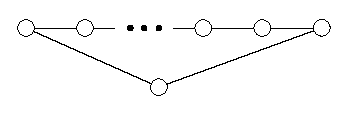
\includegraphics{table1_1(l)} & 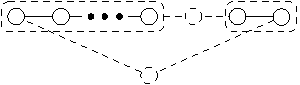
\includegraphics{table1_1(r)}
&  \\ \hline
$C_n$ & 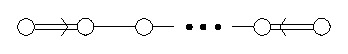
\includegraphics{table1_3(l)} & 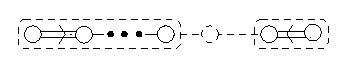
\includegraphics{table1_3(r)}
&  \\ \hline
$D_n$ & 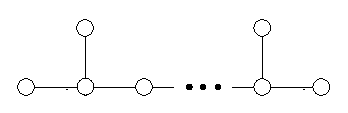
\includegraphics{table1_4(l)} & 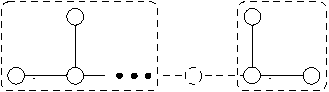
\includegraphics{table1_4(r)}
&  \\ \hline
\end{tabular}
}
\caption{Подалгебры $\af,\;\afb$ для классических серий}
\end{table}

В случае серии $B$ ситуация отличается. Причина в том, что в данном случае подалгебра $\afb$ может быть больше, чем результат удаления поддиаграммы  $\af$ и соседних вершин. Подалгебры ортогональной пары $\ \af$ и $\afb$ не обязаны образовывать прямую сумму в $\gf$. Можно явно проверить, что при  $\gf=B_{r}$ и $\af=B_{r_{\af}}$ ортогональная подалгебра -- это $\afb=B_{r-r_{\af}}$. Рассмотрим вложение $B_{r_{\af}}\rightarrow B_{r},\quad 1<r_{\af}<r$. В результате удаления простого корня  $\alpha _{r_{\af}-1}=e_{r_{\af}-1}-e_{r_{\af}}$ расширенная диаграмма Дынкина для $B_{r}$ разбивается на несвязные диаграммы $\af=B_{r_{\af}}$ и $D_{r-r_{\af}}$. Однако корневая система  $\Delta _{\afb}$ содержит не только простые корни  $\left\{ e_{1}-e_{2},e_{2}-e_{3},\ldots ,e_{r_{\af}-2}-e_{r_{\af}-1},e_{1}+e_{2}\right\} $, но и корень $e_{r_{\af}-1}$. То есть  $\Delta _{\afb}$ образует систему типа  $B_{r-r_{\af}}$ и ортогональная пара для вложения $B_{r_{\af}}\rightarrow B_{r}$ -- это  $\left( B_{r_{\af}},B_{r-r_{\af}}\right) $. В следующем разделе мы приводим пример такой ортогональной пары для вложения $B_{2}\rightarrow B_{4}$ (см. Рис. \ref{fig:dynkin}).

Полная классификация регулярных подалгебр аффинных алгебр Ли приведена в недавней работе \cite{1751-8121-41-36-365204}. Из полной классификации максимальных специальных подалгебр классических алгебр Ли \cite{dynkin1952semisimple} мы получаем следующий список пар ортогональных подалгебр $\af,\;\afb$:
\begin{equation*}
\begin{array}{lll}
su(p)\oplus su(q) & \subset su(pq) &  \\
so(p)\oplus so(q) & \subset so(pq) &  \\
sp(2p)\oplus sp(2q) & \subset so(4pq) &  \\
sp(2p)\oplus so(q) & \subset sp(2pq) &  \\
so(p)\oplus so(q) & \subset so(p+q) & \text{для нечетных}\;p\;\text{и}\;q.
\end{array}
\end{equation*}


\subsubsection{Алгоритм рекурсивного вычисления коэффициентов ветвления}

\label{sec:algorithm}

Рекуррентные соотношения (\ref{recurrent-relation}) позволяют нам сформулировать алгоритм для рекурсивного вычисления коэффициентов ветвления. При этом для работы алгоритма не требуется построение модуля $L^{(\mu)}_{\gf}$ или какого-то из модулей $L^{(\nu)}_{\af}$

Алгоритм состоит из следующих шагов:

\begin{enumerate}[(i)]
\item Построить корневую систему $\Delta _{\af}$ для вложения $\af\rightarrow \gf$.

\item Выбрать все положительные корни $\alpha \in \Delta ^{+}$, ортогональные к  $\af$, то есть сформировать множество $\Delta_{\afb }^{+}$.

\item Построить множество $\Gamma _{\af\rightarrow \gf}$. Соотношение  (\ref{eq:142}) определяет знаковую функцию $s(\gamma)$ и множество $\Phi_{\af\subset \gf}$. Вычитание наименьшего веса $\gamma_0$ дает веер вложения (\ref{fan-defined}):
 $\Gamma _{\af\rightarrow \gf}=\left\{ \xi -\gamma _{0}|\xi \in \Phi _{\af\subset \gf}\right\} \setminus \left\{ 0\right\}$.

\item Построить множество $\widehat{\Psi ^{(\mu )}}=\left\{ w (\mu +\rho
)-\rho ;\;w \in W\right\} $ сингулярных весов для  $\gf$-модуля $L^{(\mu )}$.

\item Выбрать веса $\left\{ \mu _{\widetilde{\afb}}\left( w\right) =\pi _{\widetilde{\afb}}\left[ w(\mu +\rho
)-\rho \right] -\mathcal{D}_{\afb}\in \overline{C_{\widetilde{\afb}}}\right\} $. Так как множество  $\Delta_{\afb }^{+}$ фиксировано, легко осуществить проверку принадлежности веса $\mu _{\widetilde{\afb}}\left( w\right) $ к главной камере Вейля $\overline{C_{\widetilde{\afb}}}$ (достаточно вычислить скалярные произведения с фундаментальными весами $\afb^{+}$).

\item Для весов $\mu _{\widetilde{\afb}}\left( w\right) $ вычислить размерности соответствующих модулей, $\mathrm{\dim }\left(L_{\widetilde{\afb}}^{\mu _{\widetilde{\afb}}\left( u\right) }\right) $, используя формулу Вейля для размерностей. Затем построить сингулярный элемент $\Psi ^{\left( \mu \right) }_{\left(  \af, \afb \right)}$.

\item Вычислить аномальные коэффициенты ветвления используя рекуррентное соотношение (\ref{recurrent-relation}) и выбрать среди них те, которые соответствуют весам в главной камере Вейля $\overline{C_{\af}}$.
\end{enumerate}

Можно ускорить работу алгоритма путем однократного вычисления представителей классов смежности $W/W_{\afb }$.

Следующий раздел состоит из примеров, иллюстрирующих применение данного алгоритма.

\section{Примеры}
\label{sec:branching-examples}

\subsection{Ветвления модулей конечномерных алгебр Ли}
\label{sec:finite-dimens-lie}

\subsubsection{Регулярное вложение $A_1$ в $B_2$}
\label{sec:regul-embedd-a_1}

Рассмотрим регулярное вложение $A_1\to B_2$. Простые корни $\alpha_1, \alpha_2$ алгебры $B_2$ обозначены пунктирными стрелками на Рисунке \ref{fig:B2_A1}. Мы обозначаем соответствующие элементарные отражения через $w_1, w_2$. Простой корень $\beta = \alpha_1+2\alpha_2$ алгебры $A_1$ показан серым цветом.


\begin{figure}[p]
  \noindent\centering{
    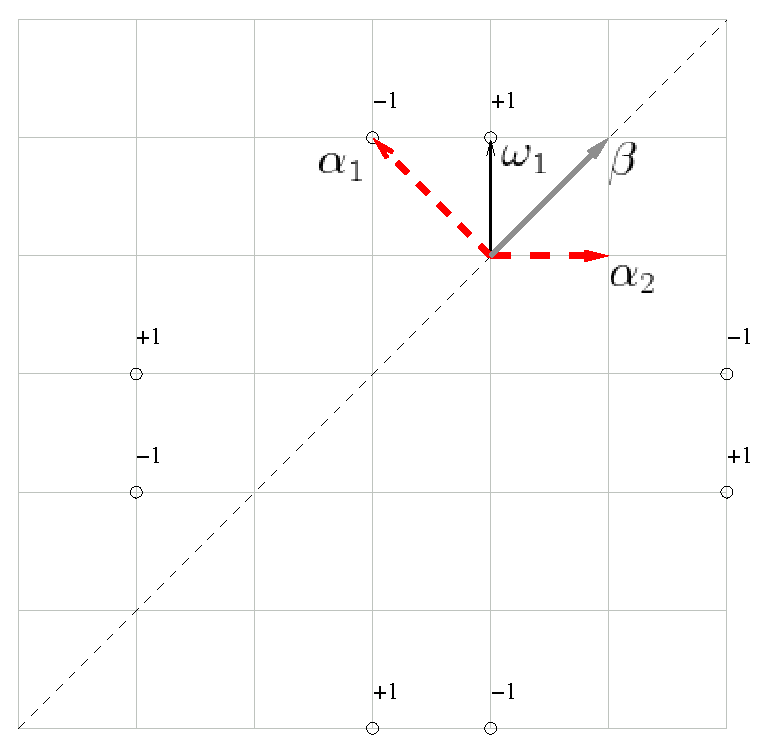
\includegraphics[width=80mm]{figure1}
  }
  \caption{Регулярное вложение  $A_1$ в $B_2$. Простые корни  $\alpha_1, \alpha_2$ алгебры $B_2$ обозначены пунктирными стрелками. Простой корень $\beta = \alpha_1+2\alpha_2$ подалгебры $A_1$ показан серым цветом. Старший вес фундаментального представления $L^{(1,0)=\omega_1}_{B_2}$ выделен черным. Веса сингулярного элемента $\Psi^{(\omega_1)}$ отмечены кругами с подписанными значениями соответствующих определителей $\epsilon(w)$.}
  \label{fig:B2_A1}

%\end{figure}
%\begin{figure}[pb]
  \noindent\centering{
    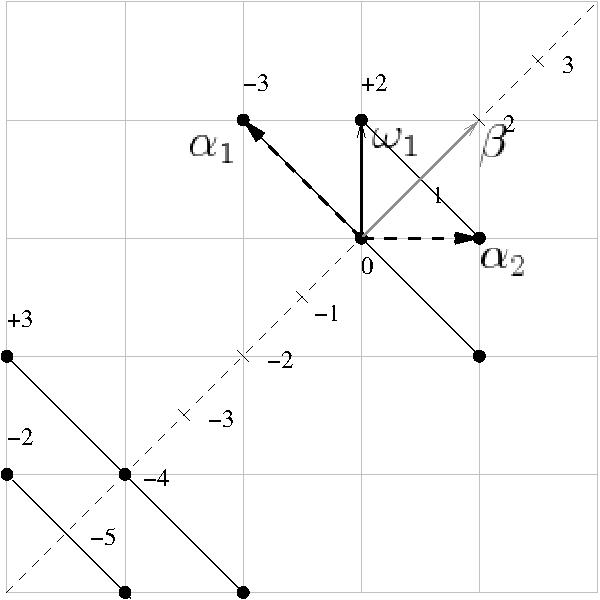
\includegraphics[width=80mm]{figure2}
  }
  \caption{Здесь диаграмма, показанная выше (Рисунок \ref{fig:B2_A1}), дополнена весами $\left( \afb=A_1 \right)$-модулей $L_{\af_{\perp }}^{\mu_{\af_{\perp }}\left( u\right) }$, построенных в точках $\pi _{\af}\left[ u(\mu +\rho )-\rho \right] $ и показанных пунктирными линиями. 
    Подписи к старшим весам   $\mu_{\af_{\perp }}\left( u\right)$ представляют собой значения произведений $\epsilon(u)\dim\left(L_{\afb}^{\mu_{\af_{\perp }}\left( u\right) }\right)$.
    Координаты вдоль корня $\beta$ указаны по отношению к фундаментальному весу $\af$. }
\label{fig:B2_A1_2}
\end{figure}

Выполним редукцию фундаментального представления  $L^{(1,0)=\omega_1}_{B_2}$ ($\omega_1$ -- черная стрелка на Рисунке \ref{fig:B2_A1}) в соответствии с алгоритмом.
Корень $\alpha_1$ ортогонален к $\beta$, так что  $\Delta_{\afb}^+ = \left\{ \alpha_1 \right\}$ (шаг (ii)).
В соответствии с Определением \ref{fan-definition} веер вложения $\Gamma_{A_1\to B_2}$ (шаг (iii)) состоит из двух весов:
\begin{equation*}
  \label{eq:22}
  \Gamma_{A_1\to B_2}=\left\{ (1;2),\; (2;-1) \right\},
\end{equation*}
где вторая компонента -- это значение знаковой функции  $s(\gamma)$.
Сингулярные веса  $\left\{ w (\omega_1 +\rho)-\rho ;\;w \in W\right\}$ (шаг (iv)) показаны кругами с подписанными значениями $\epsilon\left( w \right)$. Пространство  $U$ представляет собой факторпространство $W/W_{\afb}$, где $W_{\afb}=\left\{e,w_1\right\}$. Это означает, что сингулярные веса, находящиеся над прямой, заданной корнем $\beta$, принадлежат главной камере Вейля $\overline{C_{\widetilde{\af_{\perp }}}}$. Из формулы (\ref{defect-perp})  мы получаем  $\mathcal{D}_{\af_{\perp }}=0$ и $\hf_{\perp }=0$, то есть $\left\{ \mu _{\afb}\left( w\right)=\pi _{\afb}\left[ w(\mu +\rho)-\rho \right]\right\}$. Значит есть четыре старших веса для $\af_{\perp }$-модулей.  В базисе фундаментального веса $\frac{1}{2} \alpha_1$ алгебры $\afb$ координаты этих весов
$\left\{ \mu _{\afb}\left( u\right)=\pi _{\afb}\left[ u(\mu +\rho)-\rho \right]| u \in U \right\}$
равны
$\left\{ \left( 1\right) \left( 2\right) \left( 2\right) \left( 1\right) \right\}$ (шаг v).
На Рисунке (\ref{fig:B2_A1_2}) соответствующие весовые диаграммы
$\left\{ \mathcal{N}_{\af_{\perp }}^{\mu _{\af_{\perp }}\left( u\right) }\right\} $
построены из весов $\left\{ \mu _{\af}\left( u\right)\right\} =\left\{\pi _{\af}\left[ u(\mu +\rho )-\rho \right]\right\}
=\left\{ \left( 1\right) \left( 0\right) \left( -4\right) \left( -5\right) \right\}$ подалгебры   $\af$.
В действительности весовые диаграммы нам не нужны, достаточно знать лишь размерности модулей
$L_{\af_{\perp }}^{\mu_{\af_{\perp }}\left( u\right) }$ умноженные на
$\epsilon \left( u\right) $ (шаг vi). Полученные значения должны быть связаны с точками
$\left\{ \left( 1\right) \left( 0\right) \left( -4\right) \left( -5\right) \right\}$ в $P_{\af}$. Сингулярный элемент $\Psi ^{\left( \mu \right) }_{\left(  \af, \afb \right)}$ содержит следующий набор весов и их сингулярных кратностей:
\begin{equation}
  \label{eq:25}
  \left\{(1;2),\; (0;-3),\; (-4;3),\; (-5;-2)\right\}.
\end{equation}

Применяя формулу (\ref{recurrent-relation}) с веером
$\Gamma_{A_1\to B_2}$ к множеству (\ref{eq:25}) (шаг vii)
мы получаем нули для весов больше старшего сингулярного вектора$(1;2)$ и  $k^{(1,0)}_1=2$ для самого вектора $(1;2)$.
Для сингулярного веса $(0;-3)$ на границе $\bar{C}^{(0)}_{\af}$ рекуррентное соотношение дает
\begin{equation*}
  \label{eq:23}
  k^{(1,0)}_{0}=-1\cdot k^{(1,0)}_2 +2\cdot k^{(1,0)}_1 - 3\cdot \delta_{0,0} = 1,
\end{equation*}
и редукция завершена: $L_{B_2\downarrow A_1}^{\omega_1}=
2L_{A_1}^{\omega_{\left(A_1\right)} }
\bigoplus
L_{A_1}^{2\omega_{\left(A_1\right)} }$.

\subsubsection{Вложение  $B_2$ в $B_4$}
\label{sec:someth-high-dimens}
Рассмотрим регулярное вложение $B_2 \rightarrow B_4$. Соответствующие диаграммы Дынкина показаны на Рисунке \ref{fig:dynkin}.
\begin{figure}[h]
  \centering
  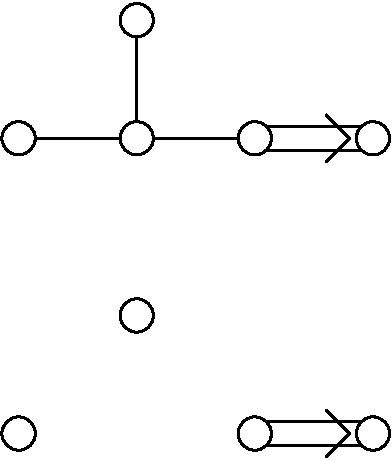
\includegraphics[width=60mm]{figure3}
  \caption{Регулярное вложение  $B_2 \rightarrow B_4$ получается путем исключения вершины из диаграммы Дынкина. 
    Напомним, что в данном случае $\afb$ равна $B_2$, тогда как на диаграмме видна только подалгебра $A_1\oplus A_1$ (см. раздел \ref{sect-embeddings}).}
  \label{fig:dynkin}
\end{figure}

\begin{figure}[pt]
  \centering
    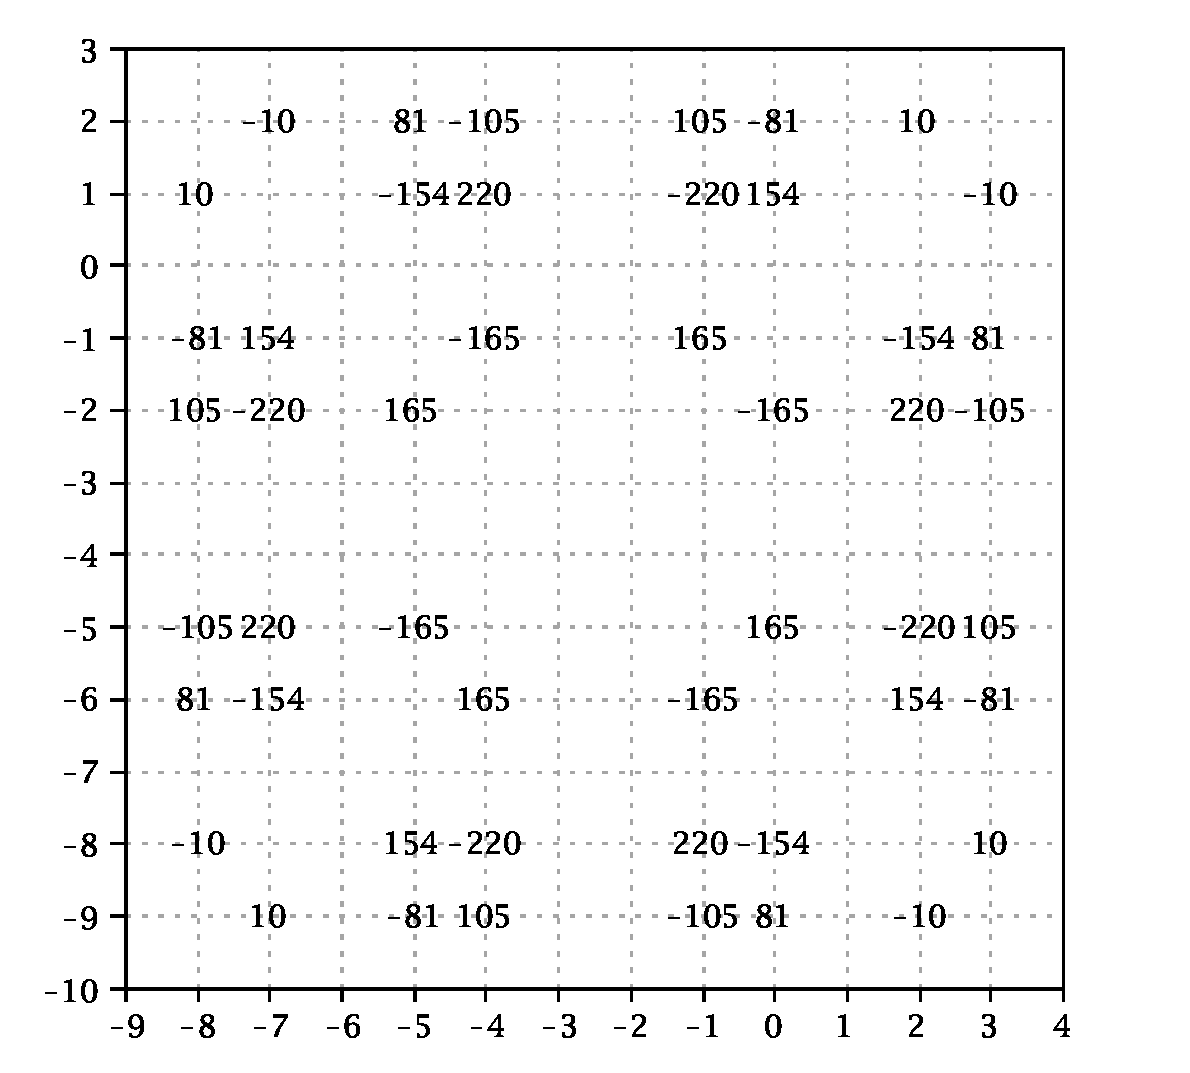
\includegraphics[width=100mm,height=90mm]{figure4}
  \caption{Сингулярный элемент  $e^{\gamma_0}\Psi ^{\left( \mu \right) }_{\left(  \af, \afb \right)}$ показан в весовом подпространстве $P_{\af}$, где $\af=B_2$ и базис равен $\left\{e_3,e_4\right\}$. Показаны спроектированные сингулярные веса $\left\{\pi _{\af}\left[ u(\mu +\rho )-\rho \right] +\gamma_0 | u \in U \right\}$, сдвинутые на  $\gamma_0$ и снабженные множителям  $\epsilon(u)\dim\left(L_{\af_{\perp }}^{\mu_{\af_{\perp }}\left( u\right) }\right)$.}
  \label{fig:B4B2anom}

%\end{figure}
%
%\begin{figure}[pb]
  \centering
  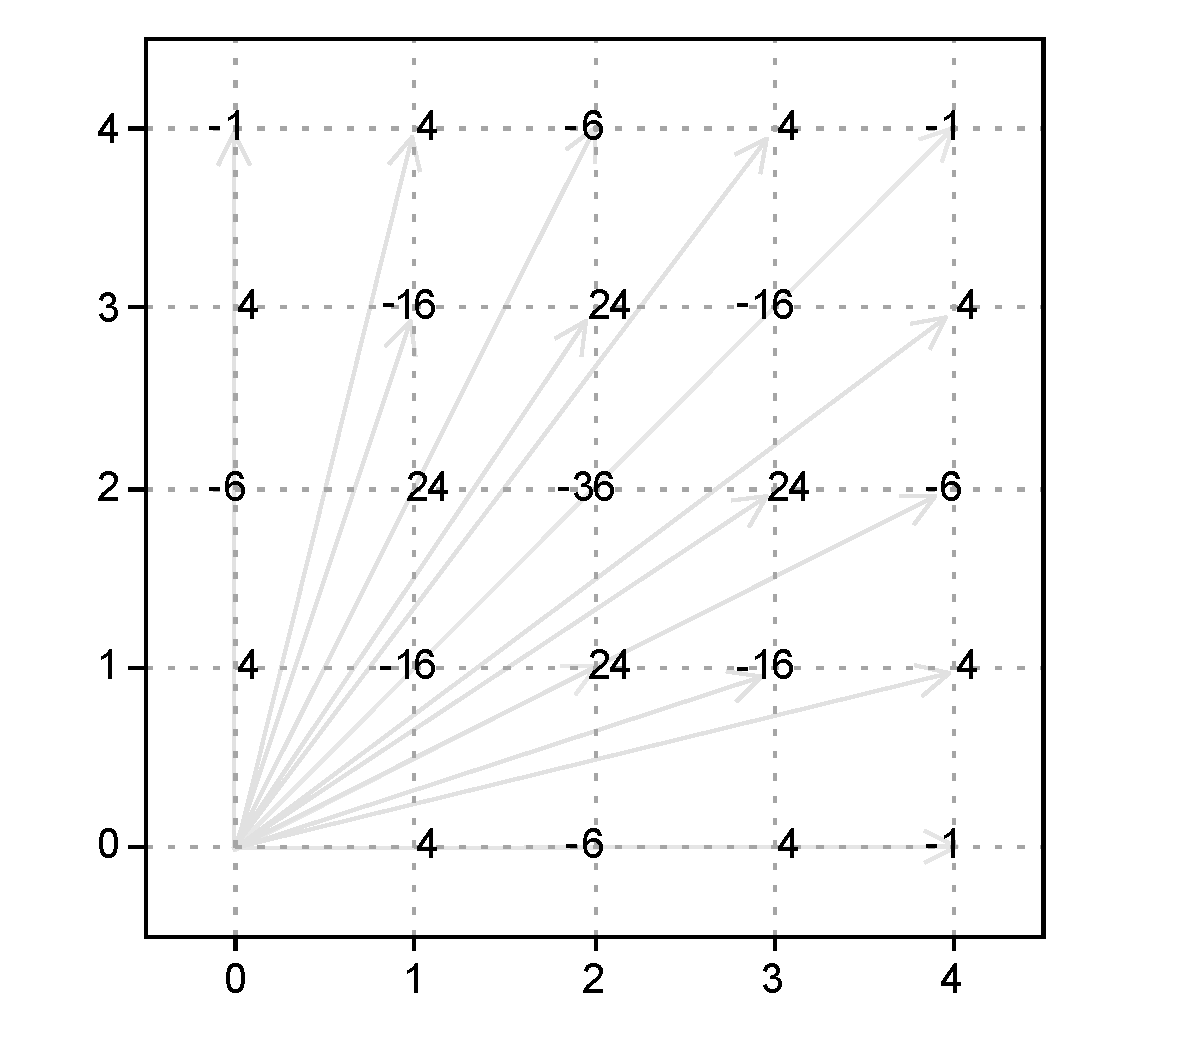
\includegraphics[height=80mm]{figure5}
  \caption{Веер $\Gamma$ для вложения $B_2\rightarrow B_4$ со значениями функции $s(\gamma+\gamma_0)$, указанными при соответствующих весах $\gamma \in \Gamma$.}
  \label{fig:B4B2Fan}
\end{figure}

В ортогональном базисе $\left\{e_1,\dots,e_4\right\}$ простые и положительные корни алгебры $B_4$ равны
\begin{eqnarray*}
  \label{eq:19}
  S_{B_4}= \{e_1 - e_2,\; e_2 - e_3,\; e_3 - e_4,\; e_4\},\\[2mm]
 \Delta^+_{B_4}=\left\{ (e_1 - e_2,\; e_2 - e_3,\; e_3 - e_4,\; e_4,\; e_1 - e_3,\; e_2 - e_4,\; e_3 + e_4,\; e_3,\; e_1 - e_4,\;\right.\\
 \left. e_2 + e_4,\; e_2,\; e_1 + e_4,\; e_2 + e_3,\; e_1,\; e_1 + e_3,\; e_1 + e_2\right\}
\end{eqnarray*}
Подалгебра  $\af=B_2$ задается простыми корнями
\begin{equation*}
  \label{eq:155}
 S_{B_2}=\{e_3-e_4,e_4\}.
\end{equation*}
Ее ортогональный партнер $\afb=B_2$ определяется корнями
\begin{eqnarray*}
  \label{eq:27}
  S_{\afb}=\{e_1-e_2,e_2\},\\
 \Delta^{+}_{\afb}= \left\{e_1-e_2,e_1+e_2,e_1,e_2\right\}.
\end{eqnarray*}
После определения множества $\Delta^+_{B_4} \setminus  \Delta^{+}_{\afb}$ можно построить веер вложения $\Gamma_{B_2 \to B_4}$ применяя Определение \ref{fan-definition}. Так как для этого вложения $s\left( \gamma_0\right)=-1$, в рекуррентном соотношении нам нужен только множитель $s\left(\gamma + \gamma_0\right)$. Результат построения веера показан на Рисунке \ref{fig:B4B2Fan}.

Рассмотрим модуль $L^{\mu}$ алгебры  $B_4$ со старшим весом $\mu=2e_1 + 2 e_2 + e_3 + e_4$; \,
$\mathrm{dim}(L^{\left[0,1,0,2\right]})=2772$.
В данном случае дефект не тривиален, $\mathcal{D}_{\af_{\perp }}=-2\left( e_1 + e_2 \right)$, тогда как $\hf_{\bot}=0$. Среди сингулярных весов есть 
48 векторов со свойством $\left\{ \mu _{\afb}\left( u\right) =\pi _{\af_{\perp }}\left[ u(\mu +\rho)-\rho \right] -\mathcal{D}_{\afb}\in \overline{C_{\afb}}\right\} $.
Таким образом мы определили множество $U=\left\{ u \right\}$. Вычислим размерности соответствующих  $\afb$-модулей со старшими весами $\mu_{\afb}\left( u\right)$ (используем формулу Вейля для размерностей) и умножим их на $\epsilon\left( u \right)$. В результате получим сингулярный элемент
$\Psi ^{\left( \mu \right) }_{\left(  \af, \afb \right)}$, показанный на Рисунке \ref{fig:B4B2anom}.

Теперь поместим веер  $\Gamma$ (см. Рисунок \ref{fig:B4B2Fan}) в старший из весов, показанных на Рисунке \ref{fig:B4B2anom} и проведем рекурсивное вычисление коэффициентов ветвления (с использованием соотношения (\ref{recurrent-relation})):
\begin{eqnarray*}
  \label{eq:24}
  \pi_{\af} \left(ch L^{\left[0,1,0,2\right]}_{B_4}\right) = 6 \; ch L^{\left[0,0\right]}_{B_2}+ 60
  \; ch L_{B_2}^{\left[0,2\right]}+ 30 \; ch L_{B_2}^{\left[1,0\right]}+ 19 \; ch L_{B_2}^{\left[2,0\right]}+\\
  40 \; ch L_{B_2}^{\left[1,2\right]}+ 10 \; ch L_{B_2}^{\left[0,4\right]}.
\end{eqnarray*}
%\newpage
\subsection{Примеры приложений в конформной теории поля}
\label{sec:phys-appl}

\subsubsection{Конформные вложения}
\label{sec:conformal-embeddings}

Как мы уже объясняли в разделе \ref{sec:modular-invariance}, коэффициенты ветвления для вложения аффинной алгебры Ли в аффинную алгебру Ли можно использовать для построения модулярно-инвариантной статсуммы для моделей Весса-Зумино-Новикова-Виттена в двумерной конформной теории поля (\cite{difrancesco1997cft}, \cite{Walton:1999xc}, \cite{walton1989conformal}, \cite{schellekens1986conformal}).
В этих моделях аффинные алгебры Ли являются алгебрами токов. 

Модулярная инвариантность статсуммы необходима для самосогласованности теории на торе и римановых поверхностях высшего рода, что важно для приложений конформной теории поля в теории струн и описании критического поведения.

Простейшая модулярно-инвариантная статсумма имеет диагональный вид:
\begin{equation}
  \label{eq:148}
   Z(\tau)=\sum_{ \mu\in P^{+}_{\mathfrak{g}}} \chi_{\mu}(\tau)\bar \chi_{\mu}(\bar \tau)
\end{equation}
Здесь суммирование ведется по множеству старших весов интегрируемых модулей в ВЗНВ-модели, а $\chi_{\mu}(\tau)$ -- это нормированные характеры (см. \cite{difrancesco1997cft}) этих модулей.

Построение недиагональных модулярных инвариантов -- это нетривиальная проблема, хотя для некоторых моделей известна полная классификация модулярных инвариантов \cite{1994hepthGannon,1995JMPGannon}.

Рассмотрим модель Весса-Зумино-Новикова-Виттена с аффинной алгеброй Ли $\af$. Недиагональные модулярные инварианты этой модели могут быть построены из диагонального инварианта, если существует аффинная алгебра  $\mathfrak{g}$, такая, что $\af\subset\mathfrak{g}$. Тогда мы можем заменить характеры  $\mathfrak{g}$-модулей в диагональной модулярно-инвариантной статсумме (\ref{eq:148}) на разложения
\begin{equation*}
  \label{eq:32}
\sum_{\nu \in P^{+}_{\af}}b^{(\mu)}_{\nu} \chi_{\nu},
\end{equation*}
содержащие нормированные характеры $\chi_{\nu}$ соответствующих $\af$-модулей. В результате мы получим недиагональную модулярно-инвариантную статсумму для теории с алгеброй токов $\af$,
\begin{equation}
  \label{eq:154}
   Z_{\af}(\tau)=\sum_{ \nu,\lambda\in P^{+}_{\af}} \chi_{\nu}(\tau)M_{\nu\lambda}\bar \chi_{\lambda}(\bar \tau).
\end{equation}

Эффективная процедура редукции существенна для этой конструкции. Вложение должно сохранять конформную инвариантность. Пусть $X^{\alpha_j}_{-n_j}$ и $\tilde{X}^{\alpha'_j}_{-n_j}$ -- понижающие операторы для алгебры $\mathfrak{g}$ и подалгебры $\af\subset\mathfrak{g}$ соответственно. Обозначим через $\pi_{\af}$ оператор проекции $\pi_{\af}:\mathfrak{g}\longrightarrow \af$. В теории, связанной с $\mathfrak{g}$ и вакуумом $\left|\lambda\right>$ состояния строятся как
\begin{equation*}
  \label{eq:151}
  X^{\alpha_1}_{-n_1}X^{\alpha_2}_{-n_2}\dots\left|\lambda\right>\quad n_1\geq n_2\geq \dots>0.
\end{equation*}
А для подалгебры $\af$ соответствующие состояния имеют вид
\begin{equation*}
  \label{eq:152}
  \tilde{X}^{\alpha'_1}_{-n_1}\tilde{X}^{\alpha'_2}_{-n_2}\dots\left|\pi_{\af}(\lambda)\right>.
\end{equation*}
Инвариантность вакуума под действием $\mathfrak{g}$ влечет его инвариантность относительно действия $\af$, но это неверно для тензора энергии-импульса. Необходимо, чтобы тензор энергии-импульса объемлющей теории содержал только генераторы $\tilde{X}$. Тогда соотношение
\begin{equation}
  \label{eq:127}
  T_{\mathfrak{g}}(z)=T_{\af}(z)
\end{equation}
ведет к равенству центральных зарядов
\begin{equation*}
  \label{eq:33}
  c(\mathfrak{g})=c(\af)
\end{equation*}
и к уравнению
\begin{equation}
  \label{eq:153}
  \frac{k\;\mathrm{dim}\,\mathfrak{g}}{k+h^{\vee}_{\gf}}=\frac{x_e k\; \mathrm{dim}\,\af}{x_ek+h^{\vee}_{\af}}.
\end{equation}
Здесь $x_e$ -- так называемый ``индекс вложения'':
$x_e=\frac{\left|\pi_{\mathfrak{a}} \theta\right|^2}{\left|\theta_{\mathfrak{a}}\right|^2}$, где $\theta$, $\theta_{\mathfrak{a}}$ -- старшие корни алгебр
$\mathfrak{g}$ и $\mathfrak{a}$, а  $h^{\vee}_{\gf}$ и $h^{\vee}_{\af}$ -- дуальные числа Кокстера.

Можно показать, что решения уравнения (\ref{eq:153}) существуют только для уровня $k=1$ \cite{difrancesco1997cft}.

Полная классификация конформных вложения дана в работе \cite{schellekens1986conformal}.

Если рассмотреть соотношение (\ref{eq:153}) и асимптотику функций ветвления, то можно доказать теорему о конечной приводимости \cite{kac1988modular}. Она утверждает, что для конформного вложения  $\af\longrightarrow\mathfrak{g}$ лишь конечное число коэффициентов ветвления отлично от нуля.

\begin{mynote} Ортогональная подалгебра  $\afb$ всегда тривиальна в случае конформного вложения $\af\longrightarrow \mathfrak{g}$.
\begin{proof}
Рассмотрим разложение тензора энергии-импульса на моды:
\begin{equation*}
\label{eq:47}
  T(z)=\frac{1}{2(k+h^v)}\sum_n z^{-n-1}L_n.
\end{equation*}
Моды $L_n$ представляют собой комбинации нормально упорядоченных произведений генераторов алгебры $\gf$,
\begin{equation*}
\label{eq:48}
  L_n=\frac{1}{2(k+h^v)}\sum_{\alpha}\sum_m:X^{\alpha}_m X^{\alpha}_{n-m}: \; .
\end{equation*}
При конформном вложении тензоры энергии-импульса  $T_{\mathfrak{g}}(z)$ и $T_{\af}(z)$ равны (см. (\ref{eq:127})).

В эти комбинации мы должны подставить генераторы подалгебры $\af$ выраженные через генераторы $\mathfrak{g}$ и получить тензор энергии-импульса $T_{\mathfrak{g}}$. Но если набор генераторов, связанных с  $\Delta_{\afb}$ не пуст, это не возможно, так как  $T_{\mathfrak{g}}$ содержит генераторы $X^{\alpha}_n$, где $\alpha\in \Delta_{\afb}$.
\end{proof}
\end{mynote}



\subsubsection{Специальное вложение $\hat{A}_1\rightarrow\hat{A}_2$.}
\label{sec:spec-embedd-hata_1s}
Рассмотрим следующие пример аффинной алгебры Ли $\gf$ и аффинной подалгебры $\af$:
$\hat{A}_1 \rightarrow \hat{A}_2$ и вложение является аффинным расширением специального вложения $A_1 \rightarrow A_2$ с индексом вложения $x_e=4$. Так как мы должны рассматривать $\gf$-модули уровня один, соответствующие  $\af$-модули будут иметь уровень $\tilde{k}=kx_e=4$.

Существует три фундаментальных веса алгебры  $\hat{A}_2$ имеющих уровень один. 
Легко видеть, что множество $\Delta_{ \afb }$ пусто и подалгебра $\afb=0$. Тогда ${\cal D}_{\afb}=0$, $\hf_{\perp}$ -- одномерная абелева подалгебра и размерность $\tilde\afb=\afb\oplus \hf_{\perp}$ также равна 1. Удобно выбрать классический корень для подалгебры $\hat{A}_1$ равным $\beta=\frac{1}{2}(\alpha_1+\alpha_2)$.

Используем Определение (\ref{fan-definition}) и построим веер $\Gamma_{\hat A_1\to\hat A_2}$. В этом случае $\gamma_0 =0$ и знак  $s\left( 0 \right)=-1$, то есть мы используем знаковую функцию $s(\gamma)$ (см. Рисунок \ref{fig:AffineA2A1Fan}).


\begin{figure}[h!bt]
  \centering
  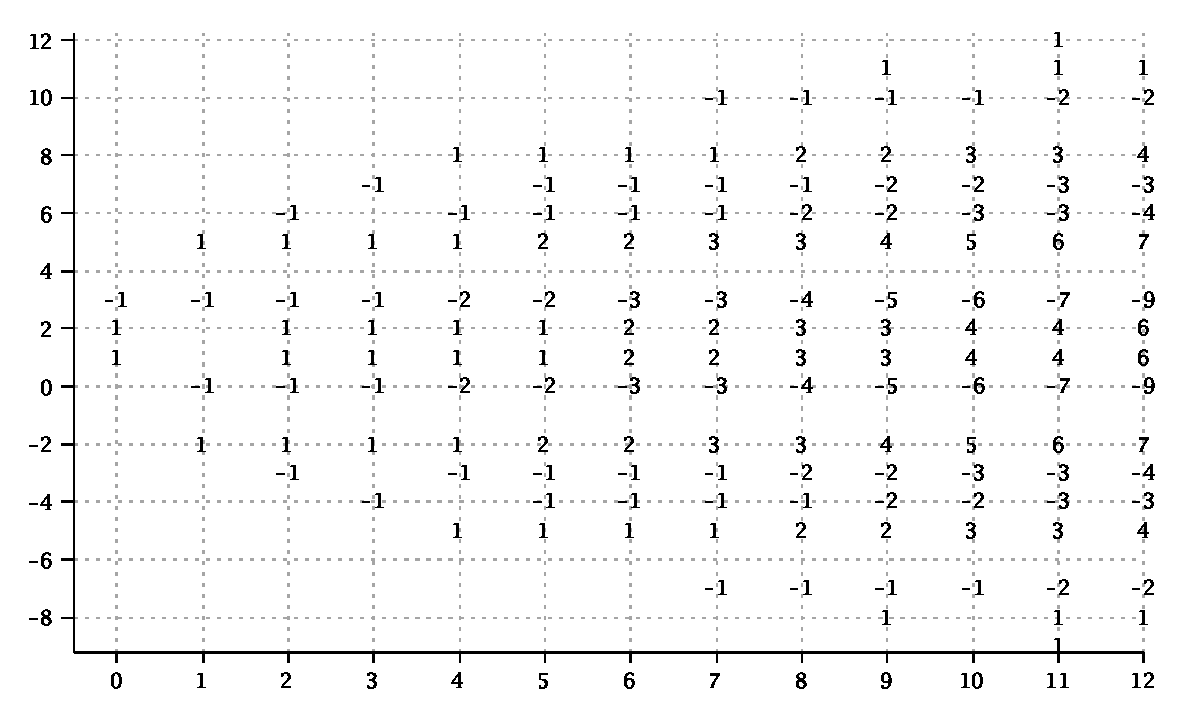
\includegraphics[width=125mm]{figure6}

  \caption{Веер  $\Gamma_{\hat{A_1}\rightarrow \hat{A_2}}$ для вложения $\hat{A_1}\rightarrow \hat{A_2}$ в базисе $\left\{\beta,\delta \right\}$. Заметим, что  $\gamma_0 =0$ и значения $s(\gamma)$ приписаны к весам $\gamma\in \Gamma_{\hat{A_1}\rightarrow \hat{A_2}}$}
  \label{fig:AffineA2A1Fan}
\end{figure}

Рассмотрим модуль $L^{\omega_0=(0,0;1;0)}$. Здесь мы используем обозначение (конечномерная часть; уровень; грейд)
для старшего веса и координаты конечномерной части даются индексами Дынкина (см. раздел \ref{sec:weights-roots}).

Множество весов $\widehat{\Psi^{(\omega_0)}}$ показано на Рисунке \ref{fig:affine_A2_anom_point} вплоть до шестого грейда.

\begin{figure}[h!tb]
  \hspace*{-1.5cm}
  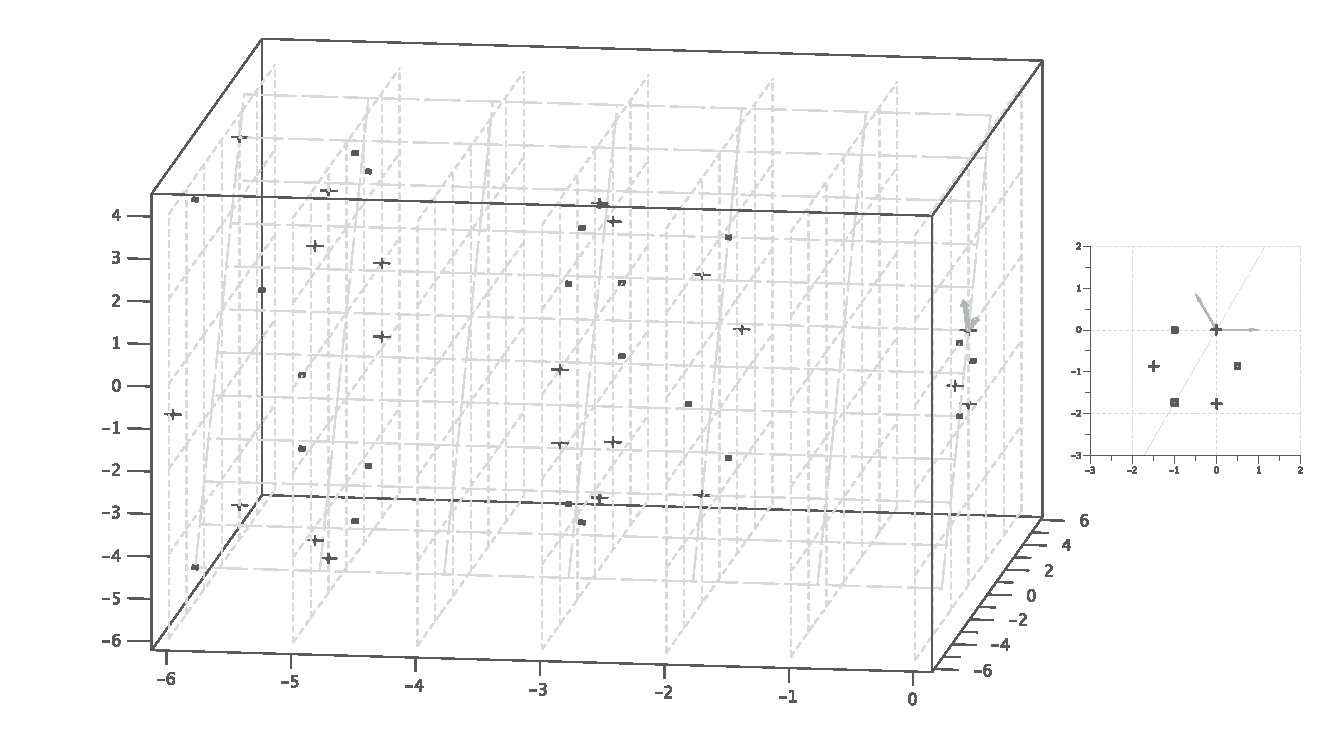
\includegraphics[width=180mm]{figure7}
  \caption{Сингулярные веса модуля $L_{\hat{A_2}}^{\omega_0}=L^{(0,0;1;0)}_{\hat{A_2}}$. Классическое сечение (нулевой грейд) диаграммы показано отдельно в правой части рисунка. 
    Мы используем ортогональный базис с единичным вектором, равным $\alpha_1$. Веса $w (\omega_0+\rho)-\rho$ показаны крестами, если $\epsilon(w)=1$ и квадратами при $\epsilon(w)=-1$. Простые корни классической подалгебры  $A_2$ показаны серым, а диагональная плоскость соответствует подалгебре Картана вложенной алгебры $\hat{A}_1$.}
  \label{fig:affine_A2_anom_point}
\end{figure}

Следующий шаг состоит в проектировании сингулярных весов на $P_{\hat A_1}$. В результате получается элемент $\Psi ^{\left( \omega_0 \right) }_{\left(  \hat A_1\, , \, \afb=0 \right)}$, изображенный на Рисунке \ref{fig:AffineA2_A1_anom_proj} вплоть до двенадцатого грейда.
\begin{figure}[h!tb]
  \centering
  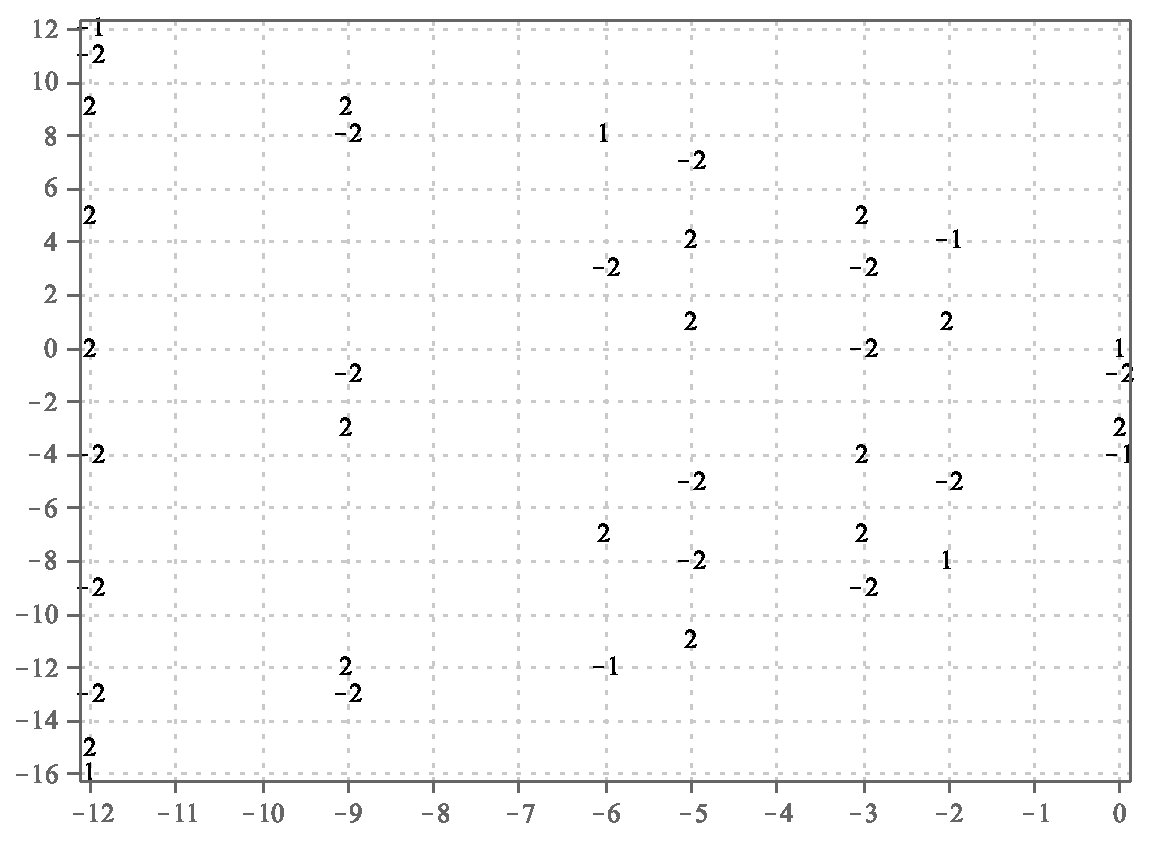
\includegraphics[width=130mm]{figure8}
  \caption{Сингулярный элемент $\Psi ^{\left( \omega_0 \right) }_{\left(  \hat A_1\, , \, \afb=0 \right)}$ показан в $P_{\hat A_1}$ с базисом $\left\{\beta,\delta \right\}$.}
  \label{fig:AffineA2_A1_anom_proj}
\end{figure}

Используя рекуррентное соотношение  (\ref{recurrent-relation}) с веером
$\Gamma_{\hat{A_1}\rightarrow \hat{A_2}}$ и сингулярными весами $\Psi ^{\left( \omega_0 \right) }_{\left(  \hat A_1\, , \, \afb=0 \right)}$, мы получаем сингулярные коэффициенты ветвления, показанные на Рисунке \ref{fig:AffineA2_A1_branching}.
\begin{figure}[h!tb]
  \centering
  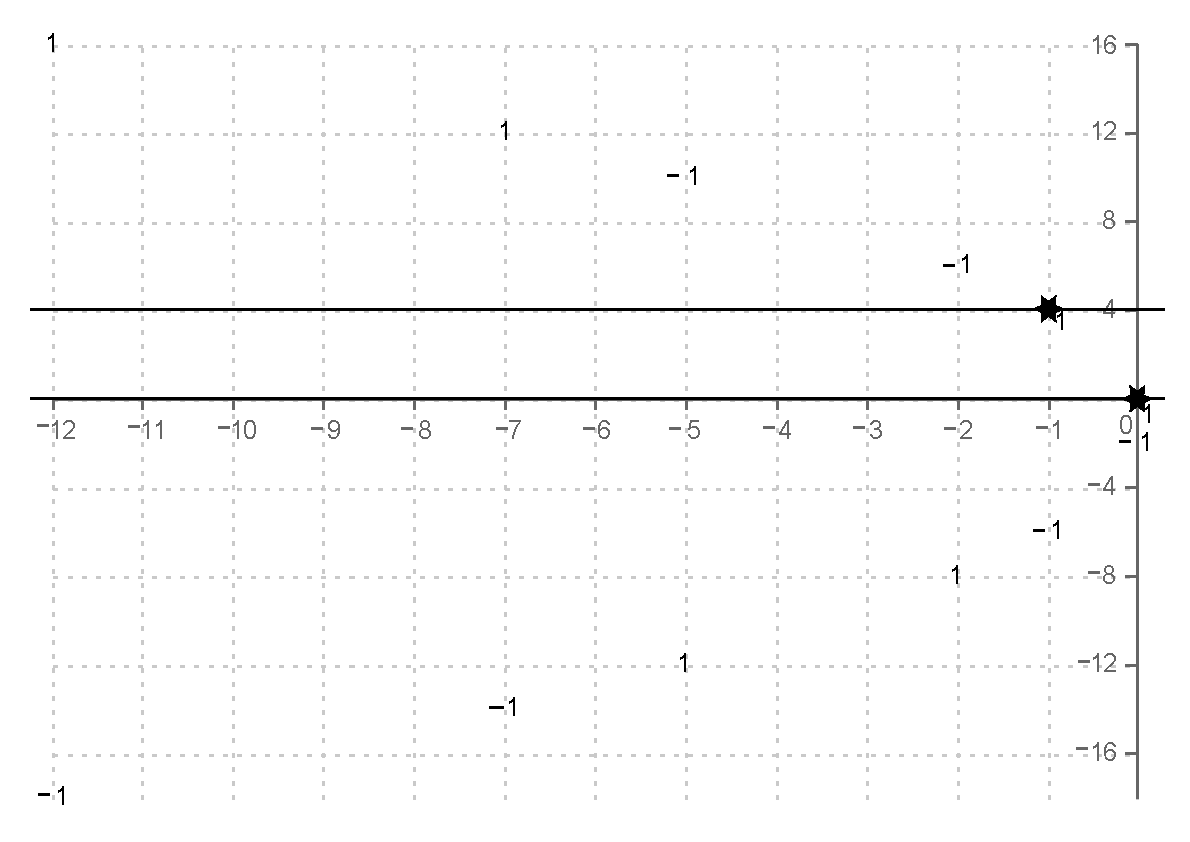
\includegraphics[width=130mm]{figure9}
  \caption{Сингулярные коэффициенты ветвления для вложения $\hat{A_1}\subset \hat{A_2}$. Границы главной камеры Вейля $\bar{C}_{\hat{A}_1}$ показаны черными линиями. Два сингулярных веса, расположенные в главной камере Вейля, отмечены звездочками. Они оба имеют кратность 1, то есть соответствующие коэффициенты ветвления равны 1.}
  \label{fig:AffineA2_A1_branching}
\end{figure}
Внутри камеры Вейля $\bar{C}_{\hat{A}_1}$ (ее границы показаны на Рисунке \ref{fig:AffineA2_A1_branching}) находятся только два ненулевых сингулярных веса и оба они имеют кратность 1. Это старшие веса подмодулей $\af$ и их кратности равны коэффициентам ветвления. То есть мы получаем разложение
\begin{equation*}
  \label{eq:43}
  L^{(0,0;1;0)}_{\hat{A_2}\downarrow \hat{A_1}}= L_{\hat{A_1}}^{(0;4;0)}\oplus L_{\hat{A_1}}^{(4;4;0)}.
\end{equation*}
Заметим, что теорема о конечной приводимости выполняется.

Тот же веер $\Gamma_{\hat{A_1}\rightarrow \hat{A_2}}$ можно использовать для других модулей старшего веса $L^{\mu}_{\hat{A_2}}$. В частности для неприводимых модулей уровня один мы получаем тривиальное ветвление:
\begin{eqnarray*}
  \label{eq:44}
   L^{(1,0;1;0)}_{\hat{A_2}\downarrow \hat{A_1}}= L_{\hat{A_1}}^{(2;4;0)},\\
   L^{(0,1;1;0)}_{\hat{A_2}\downarrow \hat{A_1}}= L_{\hat{A_1}}^{(2;4;0)}.
\end{eqnarray*}

Используя эти результаты легко получить модулярно-инвариантную статсумму:
\begin{equation*}
  \label{eq:45}
  Z=\left|\chi_{(4;4;0)}+\chi_{(0;4;0)}\right|^2+2\chi_{(2;4;0)}^2.
\end{equation*}

\subsubsection{Coset-модели}
\label{sec:coset-models}

Coset-модели \cite{Goddard198588}, тесно связанные с калибровочными ВЗНВ-моделями, активно изучаются в теории струн, особенно в струнных моделях в пространстве анти де Ситтера
\cite{Maldacena:2000hw,Maldacena:2000kv,Maldacena:2001km,Maldacena:2001ky,Aharony:1999ti}. Характеры в coset-моделях пропорциональны функциям ветвления.
\begin{equation}
  \label{eq:31}
  \chi^{(\mu)}_{\nu}(\tau)=e^{2\pi i \tau (m_{\mu}-m_{\nu})} b^{(\mu)}_{\nu}(\tau),
\end{equation}
где
\begin{equation*}
  \label{eq:46}
  m_{\mu}=\frac{\left|\mu+\rho\right|^2}{2(k+g)}-\frac{\left|\rho\right|^2}{2g}.
\end{equation*}
Проблема построения функций ветвления для  coset-моделей рассматривалась в работах  \cite{Dunbar:1992gh}, \cite{Hwang:1994yr}, \cite{lu1994branching}.

Вернемся к нашему примеру \ref{sec:regul-embedd-a_1} и рассмотрим аффинное расширение вложения $A_1 \rightarrow B_2$. Так как вложение регулярно и индекс $x_e=1$, модули подалгебры и исходный модуль имеют одинаковый уровень. Множество положительных корней с нулевой проекцией на корневое пространство подалгебры  $\hat{A_1}$ то же, что и в конечномерном случае: $\Delta^{+}_{\afb}=\left\{ \alpha_1 \right\}$ и $\afb=A_1$. Легко видеть, что здесь $\hf_{\perp}$ тривиальна и  ${\cal D}_{\afb}=0$.

Используя Определение \ref{fan-definition} мы получаем веер вложения $\Gamma_{\hat{A_1} \longrightarrow  \hat{B_2} }$. Заметим, что наименьший вес веера $\gamma_0$ равен нулю и  $s\left( \gamma_0 \right)=-1$. Значения знаковой функции  $s(\gamma)$ для $ \gamma \in \Gamma_{\hat{A_1} \longrightarrow  \hat{B_2} }$ показаны на Рисунке \ref{fig:AffineB2A1Fan}.
Мы ограничили вычисление двенадцатым грейдом. 
\begin{figure}[h!bt]
  \centering
  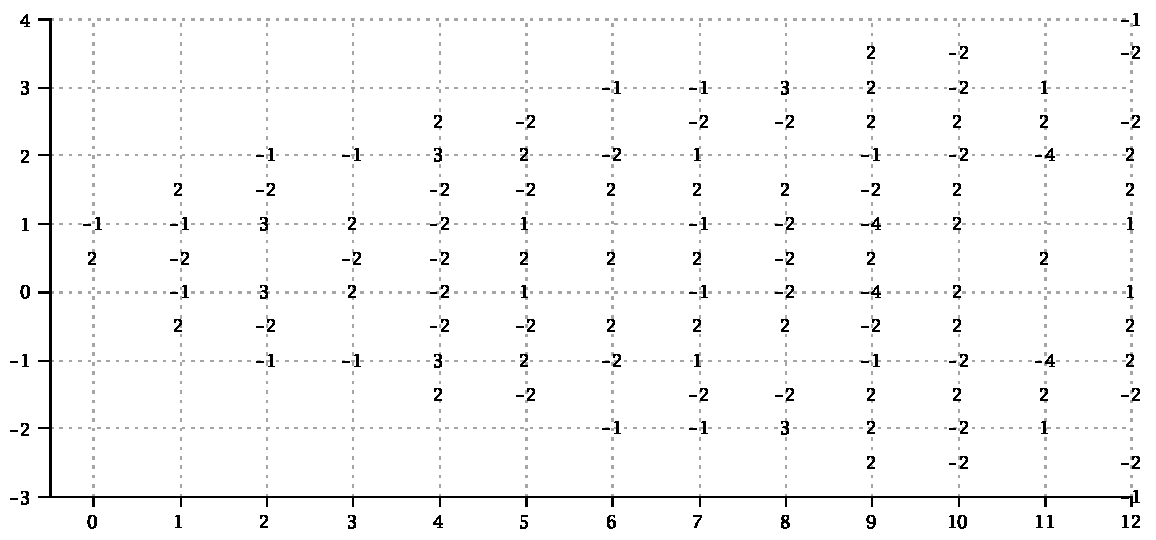
\includegraphics[width=135mm]{figure10}
  \caption{Веер $\Gamma_{\hat{A_1}\rightarrow \hat{B_2}}$ для вложения $\hat{A_1}\rightarrow \hat{B_2}$ в базисе $\left\{\beta,\delta \right\}$. Значения $s(\gamma)$ показаны для весов $\gamma\in \Gamma_{\hat{A_1}\rightarrow \hat{B_2}}$}
  \label{fig:AffineB2A1Fan}
\end{figure}

Рассмотрим модуль уровня один $L^{\left( 1,0;1;0 \right)}_{\hat{B_2}}$  со старшим весом  $\omega_1=(1,0;1;0)$, где координаты конечномерной части даны в ортогональном базисе $e_1,e_2$. Множество сингулярных весов для этого модуля вплоть до шестого грейда приведено на Рисунке \ref{fig:affine_B2_anom_point}.

\begin{figure}[h!tb]
%  \hspace*{-2cm}
  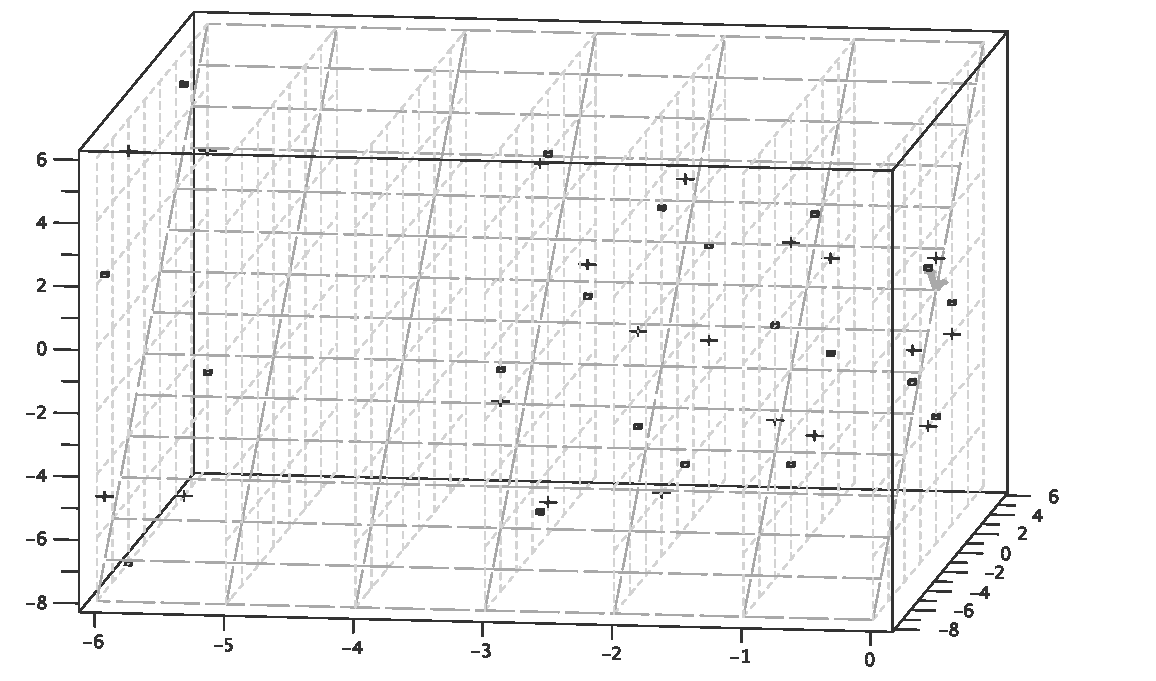
\includegraphics[width=140mm]{figure11}
  \caption{Сингулярные веса модуля $L^{(1,0;1;0)}_{\hat B_2 }$. В классическом сечении используется стандартный базис  $\{e_1,e_2\}$. Веса в нулевом грейде те же, что и на Рисунке \ref{fig:B2_A1}. Веса  $w (\omega_1+\rho)-\rho$ отмечены крестами, если $\epsilon(w)=1$ и квадратами при $\epsilon(w)=-1$. Простые корни классической подалгебры  $B_2$ показаны серым, а диагональная плоскость соответствует подалгебре Картана вложенной алгебры $\hat{A}_1$.}
  \label{fig:affine_B2_anom_point}
\end{figure}

В соответствии с рекурсивным алгоритмом  \ref{sec:algorithm} мы проектируем сингулярные веса на $P_{\hat{A_1}}$ и вычисляем размерности $\afb$-модулей $L^{\pi_{\afb}(w(\mu+\rho))-\rho_{\afb}}_{\afb}$. В нулевом грейде эта проекция дает в точности множество $\Psi ^{\left( \mu \right) }_{\left(  A_1, A_1 \right)}$, соответствующее вложению классической алгебры Ли  $A_1\rightarrow B_2$. Это можно заметить сравнивая Рисунок \ref{fig:B2_A1} и Рисунок \ref{fig:AffineB2_A1_anom_proj}, на котором сингулярный элемент $\Psi ^{\left( \mu \right) }_{\left(  \widehat{A_1}, A_1 \right)}$ для аффинного вложения  $\hat{A_1}\to\hat{B_{2}}$  показан вплоть до двенадцатого грейда.
\begin{figure}[h!tb]
  \centering
  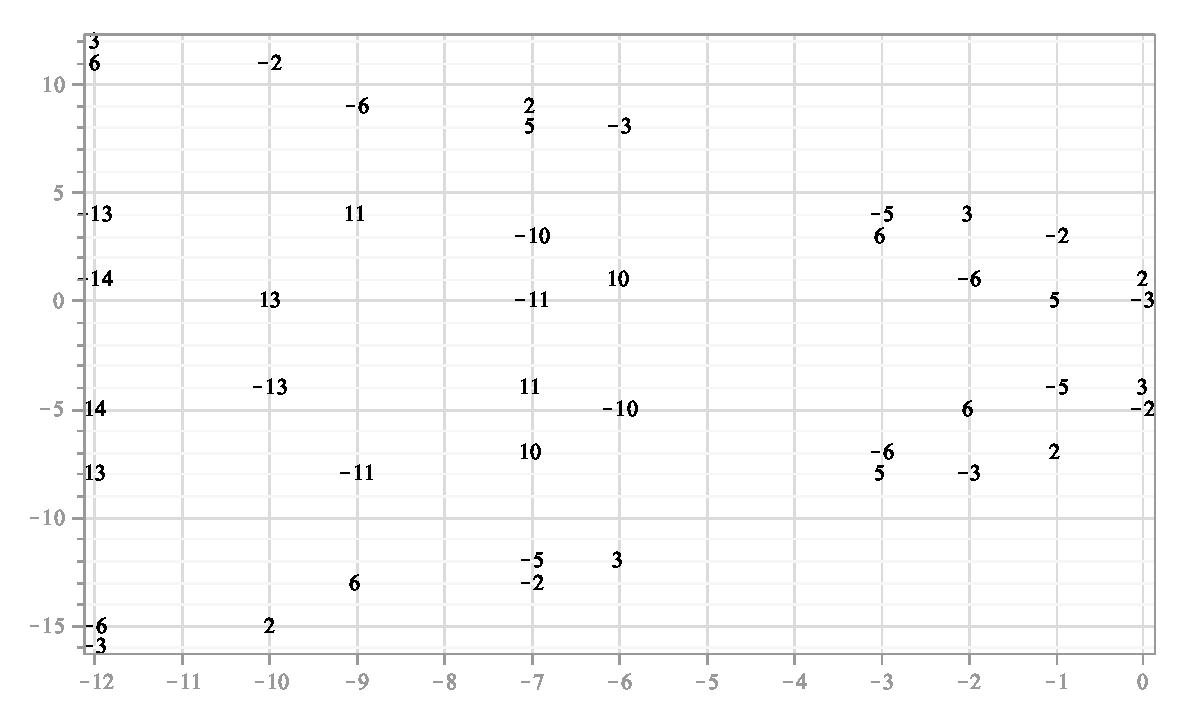
\includegraphics[width=120mm]{figure12}
  \caption{Сингулярный элемент $\Psi ^{\left( \omega_1 \right) }_{\left(  \widehat{A_1}, A_1 \right)}$ в базисе $\{\beta,\delta\}$. Размерности соответствующих  $\afb=A_1$-модулей со знаками  $\epsilon(u)$ представлены на рисунке.}
  \label{fig:AffineB2_A1_anom_proj}
\end{figure}

\begin{figure}[h!bt]
  \centering
  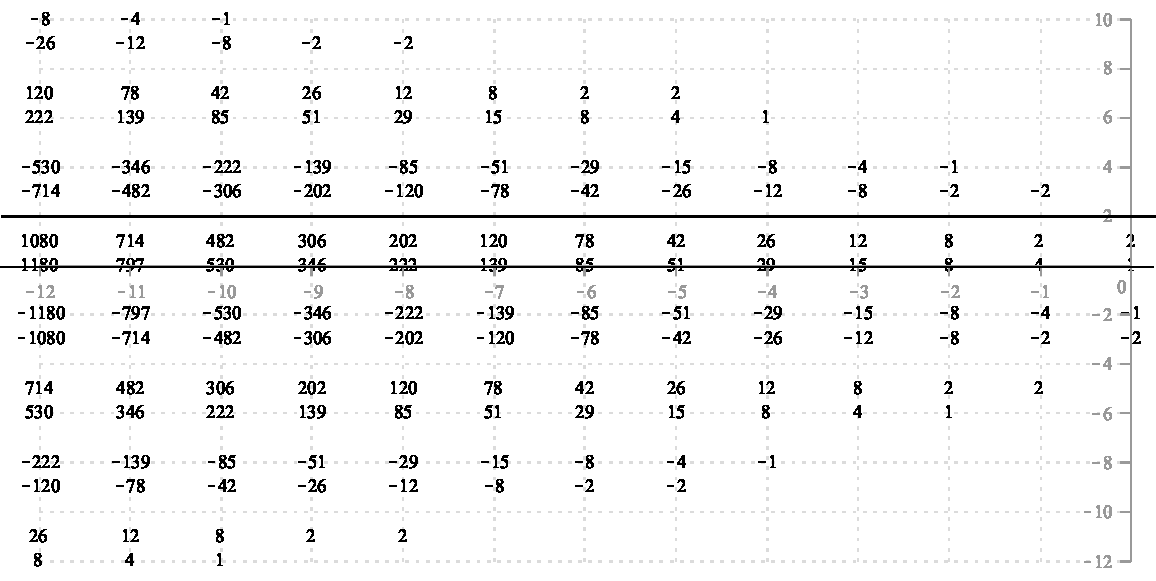
\includegraphics[width=120mm]{figure13}
  \caption{Сингулярные коэффициенты ветвления для вложения $\hat{A_1}\rightarrow \hat{B_2}$. Использован базис $\{\beta,\delta\}$. Границы главной камеры Вейля $\bar{C}_{\hat{A}_1}$ показаны черными линиями. Сингулярные коэффициенты ветвления внутри главной камеры Вейля равны коэффициентам ветвления для вложения $\hat{A_1}\rightarrow \hat{B_2}$.}
  \label{fig:AffineB2_A1_branching}
\end{figure}

Кратности старших весов внутри главной камеры Вейля
$\bar{C}^{\left( 0 \right)}_{\hat{A_1}}$ определяют следующие значения коэффициентов ветвления (до двенадцатого грейда):
\begin{eqnarray*}
  \label{eq:28}
  L^{\omega_1}_{\hat{B_2}\downarrow \hat{A_1}}
  &=&2 L_{\hat{A_1}}^{\omega_1}\oplus 1 L_{\hat{A_1}}^{\omega_0}\oplus 4 L_{\hat{A_1}}^{\omega_0-\delta}\oplus\\
    &&2 L_{\hat{A_1}}^{\omega_1-\delta}\oplus 8 L_{\hat{A_1}}^{\omega_0-2\delta}\oplus
    8 L_{\hat{A_1}}^{\omega_1-2\delta}\oplus 15 L_{\hat{A_1}}^{\omega_0-3\delta}\oplus\\
    &&12 L_{\hat{A_1}}^{\omega_1-3\delta}\oplus 26 L_{\hat{A_1}}^{\omega_1-4\delta}\oplus
    29 L_{\hat{A_1}}^{\omega_0-4\delta}\oplus 51 L_{\hat{A_1}}^{\omega_0-5\delta}\oplus\\
    &&42 L_{\hat{A_1}}^{\omega_1-5\delta}\oplus 78 L_{\hat{A_1}}^{\omega_1-6\delta}\oplus
    85 L_{\hat{A_1}}^{\omega_0-6\delta}\oplus 120 L_{\hat{A_1}}^{\omega_1-7\delta}\oplus\\
    &&139 L_{\hat{A_1}}^{\omega_0-7\delta}\oplus 202 L_{\hat{A_1}}^{\omega_1-8\delta}\oplus
    222 L_{\hat{A_1}}^{\omega_0-8\delta}\oplus 306 L_{\hat{A_1}}^{\omega_1-9\delta}\oplus\\
    &&346 L_{\hat{A_1}}^{\omega_0-9\delta}\oplus 530 L_{\hat{A_1}}^{\omega_0-10\delta}\oplus
    482 L_{\hat{A_1}}^{\omega_1-10\delta}\oplus 714 L_{\hat{A_1}}^{\omega_1-11\delta}\oplus\\
    &&797 L_{\hat{A_1}}^{\omega_0-11\delta}\oplus 1080 L_{\hat{A_1}}^{\omega_1-12\delta}\oplus
    1180 L_{\hat{A_1}}^{\omega_0-12\delta}\oplus \dots
\end{eqnarray*}
Этот результат можно представить в виде набора функций ветвления:
\begin{eqnarray*}
  \label{eq:29}
  \begin{array}{cc}
    b^{(\omega_1)}_{0}= & 1 + 4\,q^{1}+ 8\,q^{2}+ 15\,q^{3}+ 29\,q^{4}+ 51\,q^{5}+ 85\,q^{6}+ 139\,q^{7}+\\
     &222\,q^{8}+ 346\,q^{9}+ 530\,q^{10}+ 797\,q^{11}+ 1180\,q^{12}+\dots\\
  \end{array}\\
  \begin{array}{cc}
    b^{(\omega_1)}_{1}= &2+2\,q^{1}+8\,q^{2}+12\,q^{3}+26\,q^{4}+42\,q^{5}+78\,q^{6}+120\,q^{7}+\\
    & 202\,q^{8}+306\,q^{9}+482\,q^{10}+714\,q^{11}+1080\,q^{12}+\dots
  \end{array}
\end{eqnarray*}
Здесь $q=\exp (2\pi i \tau)$ и нижний индекс нумерует функции ветвления по их старшим весам в  $P^+_{\hat{A_1}}$, равным фундаментальным весам $\omega_0=\lambda_0=(0,1,0),\; \omega_1=\alpha/2=(1,1,0)$.

Теперь мы можем вернуться к равенству (\ref{eq:31}) и получить выражение для характеров coset-модели $B_2/A_1$:
\begin{equation*}
  \label{eq:35}
  \begin{array}{cc}
    \chi^{(\omega_1)}_{1}(q)= & q^{\frac{7}{12}}\left( 2+2\,q^{1}+8\,q^{2}+12\,q^{3}+26\,q^{4}+42\,q^{5}+78\,q^{6}+120\,q^{7}+\right. \\
    & \left. 202\,q^{8}+306\,q^{9}+482\,q^{10}+714\,q^{11}+1080\,q^{12}+\dots \right),\\
    \chi^{(\omega_1)}_{0}(q) = & q^{\frac{5}{6}}\left(1 + 4\,q^{1}+ 8\,q^{2}+ 15\,q^{3}+ 29\,q^{4}+ 51\,q^{5}+ 85\,q^{6}+ 139\,q^{7}+\right. \\
    &\left. 222\,q^{8}+ 346\,q^{9}+ 530\,q^{10}+ 797\,q^{11}+ 1180\,q^{12}+\dots\right).
  \end{array}
\end{equation*}

\section{Заключение}
\label{sec:conclusion}

Мы продемонстрировали, что техника веера вложения может использоваться для работы с произвольными редуктивными подалгебрами (как максимальными, так и не максимальными). Также показано, что проблема редукции для  $\af \subset \gf$ тесно связана со свойствами ортогонального партнера $ \afb $ подалгебры $\af$. Подалгебра  $\afb$ соответствует подмножеству положительных корней $\Delta^{+}_{\afb}$ в $\Delta_{\mathfrak{g}}^{+}$, которое тривиализует подалгебру Картана $\hf_{\afb}$. Веер вложения и множества сингулярных весов для модулей старшего веса алгебры $\gf$ существенным образом зависят от структуры  $\afb$ и ее подмодулей.  Для веера  $\Gamma_{\af\rightarrow \gf}$ эта зависимость почти очевидна: в элементе  $\Phi_{\af\rightarrow \gf}$ исключены множители, соответствующие корням  $\Delta^{+}_{\afb}$. Преобразование множества спроектированных сингулярных весов более интересно. Мы показали, что в новом сингулярном элементе $\Psi ^{\left( \mu \right) }_{\left(  \af, \afb \right)}$ коэффициенты зависят от $\afb$-подмодулей (их старшие веса $\mu _{\widetilde{\afb}}\left( u\right)$ заданы вложением и весами первоначального элемента $\Psi^{\mu}$). К счастью, для вычислений не требуется никакой информации о  $L^{\mu _{\widetilde{\afb}}\left( u\right)}_{\left\{ \afb \right\}}$-подмодулях, кроме их размерностей. В новом сингулярном элементе $\Psi ^{\left( \mu \right) }_{\left(  \af, \afb \right)}$ кратности весов равны размерностям $\dim\left(L^{\mu _{\widetilde{\afb}}\left( u\right)}_{\left\{ \afb \right\}}\right)$ соответствующих  $\afb$-модулей, умноженным на значения $\epsilon (u)$. В результате старшие веса подмодулей $\af$ и их кратности удовлетворяют набору линейных соотношений (\ref{eq:121}). Эти свойства выполняются для любой редуктивной подалгебры $\af\rightarrow \gf$ и уравнения могут быть переписаны в виде рекуррентных соотношений, которые можно решать последовательно.

Эффективность полученного алгоритма была продемонстрирована на различных примерах. В частности, мы рассмотрели построение модулярно-инвариантных статсумм в методе конформных вложений и coset-конструкцию моделей рациональной конформной теории поля. Эти конструкции полезны при изучении ВЗНВ-моделей, возникающих в контексте AdS/CFT соответствия \cite{Maldacena:2000hw,Maldacena:2000kv,Maldacena:2001km}.

Дальнейшее улучшение алгоритма может быть достигнуто при использовании техники сложенных вееров \cite{il2010folded}. Нужно отметить, что даже в случае струнных функций явное решение соответствующих рекуррентных соотношений представляет собой сложную проблему (см. подробности в работе\cite{il2010folded}). Тем не менее, мы надеемся, что развитие процедуры сложения позволит получить явные решения хотя бы для некоторых функций ветвления и соответствующих характеров coset-моделей.

%-----------------------------------------------------------------------------------------------------



%%
%% End of file
%%% Local Variables: 
%%% mode: latex
%%% TeX-master: "thesis"
%%% End: 
